\documentclass[UTF8,a4paper,12pt]{ctexart}
% Adapted from supplied lab4_mpi_report/main.tex; experiment contents not copied.


\usepackage[a4paper,margin=2.4cm,headheight=15pt]{geometry}
\usepackage{graphicx}
\usepackage{booktabs}
\usepackage{tabularx}
\usepackage{array}
\usepackage{amsmath}
\usepackage{amssymb}
\usepackage{float}
\usepackage{subcaption}
\usepackage[table]{xcolor}
\usepackage{listings}
\usepackage{fancyhdr}
\usepackage{caption}
\usepackage{enumitem}
\usepackage{makecell}
\usepackage{siunitx}
\usepackage{titlesec}
\usepackage{hyperref}
\usepackage{tikz}
\usetikzlibrary{arrows.meta,positioning,fit}
\usepackage{needspace}
\AddToHook{cmd/section/before}{\Needspace{9\baselineskip}}
\AddToHook{cmd/subsection/before}{\Needspace{4\baselineskip}}
\AddToHook{cmd/subsubsection/before}{\Needspace{4\baselineskip}}
\newcolumntype{L}[1]{>{\raggedright\arraybackslash}p{#1}}
\newcolumntype{Y}{>{\raggedright\arraybackslash}X}
\raggedbottom

\hypersetup{colorlinks=true,linkcolor=black,citecolor=black,urlcolor=blue}
\setlist[itemize]{leftmargin=2em,itemsep=0.25em,topsep=0.25em}
\setlist[enumerate]{leftmargin=2em,itemsep=0.25em,topsep=0.25em}
\captionsetup{font=small,labelfont=bf,skip=3pt}
\setlength{\abovecaptionskip}{3pt}
\setlength{\belowcaptionskip}{3pt}
\setlength{\textfloatsep}{8pt plus 2pt minus 2pt}
\setlength{\floatsep}{6pt plus 2pt minus 2pt}
\setlength{\intextsep}{6pt plus 2pt minus 2pt}
\renewcommand{\topfraction}{0.92}
\renewcommand{\bottomfraction}{0.82}
\renewcommand{\textfraction}{0.06}
\renewcommand{\floatpagefraction}{0.80}
\setlength{\abovedisplayskip}{6pt plus 1pt minus 1pt}
\setlength{\belowdisplayskip}{6pt plus 1pt minus 1pt}
\setlength{\emergencystretch}{2.5em}
\hfuzz=0pt
\titlespacing*{\section}{0pt}{1.0ex plus 0.2ex minus 0.1ex}{0.75ex}
\titlespacing*{\subsection}{0pt}{0.85ex plus 0.2ex minus 0.1ex}{0.50ex}
\titlespacing*{\subsubsection}{0pt}{0.65ex plus 0.1ex minus 0.1ex}{0.40ex}
\renewcommand{\arraystretch}{1.18}

\definecolor{nkuPurple}{RGB}{121,42,104}
\definecolor{blueGray}{RGB}{71,96,121}
\definecolor{tableHead}{RGB}{241,232,239}
\definecolor{codebg}{RGB}{255,247,236}
\definecolor{codeframe}{RGB}{232,156,78}
\definecolor{bestCell}{RGB}{255,243,214}
\definecolor{noteBg}{RGB}{245,248,252}
\definecolor{softBlue}{RGB}{235,241,248}

\lstdefinestyle{codebox}{
  backgroundcolor=\color{codebg},
  frame=single,
  rulecolor=\color{codeframe},
  basicstyle=\ttfamily\footnotesize,
  keywordstyle=\color{blue!70!black},
  commentstyle=\color{green!45!black},
  stringstyle=\color{purple!70!black},
  breaklines=true,
  breakatwhitespace=false,
  columns=fullflexible,
  keepspaces=true,
  showstringspaces=false,
  numbers=left,
  numberstyle=\tiny\color{gray},
  xleftmargin=1.5em,
  framexleftmargin=1.2em,
  aboveskip=0.25em,
  belowskip=0.25em
}
\lstset{style=codebox}

\renewcommand{\thesection}{\chinese{section}}
\renewcommand{\thesubsection}{（\chinese{subsection}）}
\renewcommand{\thesubsubsection}{\arabic{subsubsection}.}
\titleformat{\section}{\centering\zihao{3}\bfseries}{\thesection、}{0.25em}{}
\titleformat{\subsection}{\zihao{4}\bfseries}{\thesubsection}{0.25em}{}
\titleformat{\subsubsection}{\bfseries}{\thesubsubsection}{0.25em}{}

\pagestyle{fancy}
\fancyhf{}
\lhead{编译原理预备实验}
\rhead{LLVM IR 与 RISC-V 编程}
\cfoot{\thepage}

\newcommand{\figdir}{figures}
\newcommand{\metric}[1]{\textsf{#1}}
\newcommand{\codefile}[1]{\path{#1}}


\usepackage{longtable}
\usepackage{xurl}
\setcounter{tocdepth}{3}
% Member identity and division of work are confirmed by the group.
\newcommand{\MemberOne}{朱泽帅}
\newcommand{\StudentOne}{2411560}
\newcommand{\MemberTwo}{张宸笛}
\newcommand{\StudentTwo}{2412565}
\newcommand{\ExperimentDate}{2026 年 10 月 3 日}

\begin{document}
\hypersetup{pageanchor=false}
\begin{titlepage}
\thispagestyle{empty}
\centering
\vspace*{0.65cm}
\includegraphics[width=0.48\textwidth]{figures/nku.png}
\vspace{1.1cm}

{\color{nkuPurple}\rule{0.72\textwidth}{1.1pt}}\par
\vspace{0.48cm}
{\zihao{3}\bfseries 计算机学院\quad 编译原理}\par
\vspace{0.68cm}
{\zihao{2}\bfseries 预备工作：了解你的编译器}\par
\vspace{0.34cm}
{\zihao{3}\bfseries LLVM IR 编程与汇编编程}\par
\vspace{0.4cm}
{\zihao{-4}完整工具链、语义等价实现与 AscendNPU IR 探索}\par
\vspace{0.5cm}
{\color{nkuPurple}\rule{0.72\textwidth}{1.1pt}}\par
\vspace{1.35cm}
\renewcommand{\arraystretch}{1.55}
\begin{tabularx}{0.76\textwidth}{>{\zihao{4}\bfseries\raggedleft\arraybackslash}p{2.7cm}X}
小组成员 & \MemberOne\quad\StudentOne \\
小组成员 & \MemberTwo\quad\StudentTwo \\
目标架构 & RISC-V RV64GC / LP64D \\
执行环境 & WSL2 + QEMU 用户态模拟 \\
报告性质 & 双人小组共同报告 \\
\end{tabularx}
\renewcommand{\arraystretch}{1.18}
\vfill
{\color{nkuPurple}\rule{0.24\textwidth}{0.8pt}}\par
\vspace{0.35cm}
{\zihao{4}\ExperimentDate}
\end{titlepage}
\pagenumbering{Roman}
\hypersetup{pageanchor=true}
\section*{成员分工}

\textbf{朱泽帅}主要负责完整编译工具链实验及 LLVM IR 编程部分，包括 GCC/Clang 预处理、编译、汇编和链接各阶段的功能与产物分析，不同优化选项下的中间代码和目标代码比较，以及 SysY 示例程序的 LLVM IR 等价实现、控制流图（CFG）、静态单赋值形式（SSA）、短路求值和数组寻址等机制分析。

\textbf{张宸笛}主要负责 RISC-V 汇编编程部分，包括 SysY 示例程序的 RISC-V 汇编等价实现、整数与浮点运算、条件分支与循环、函数调用、LP64D ABI、寄存器分配与保存、栈帧组织，以及汇编程序的构建与执行分析。

\textbf{进阶实验由两人共同完成}，包括 AscendNPU IR 实验环境配置、官方 VecAdd 示例研究、MLIR 中端逐层 lowering 过程分析，以及核类型推导、UB 内存规划、跨流水同步、模板转换和设备后端限制等内容的探索与验证。

此外，两人共同设计 SysY 示例程序并确定语言特性覆盖范围，共同完成 SysY 运行时库链接、三种实现的构建与语义等价验证、测试结果分析，并合作完成实验报告的撰写、图表整理、结论讨论与最终审阅。

\section*{摘要}
本实验分析完整编译工具链，并对两个互补的 SysY 示例分别手写 LLVM IR 与 RISC-V 汇编。工具链部分比较 GCC/Clang 的 O0、O2 与 O2-g 六种构建，60 次运行均符合预期；Clang 的向量化伴随代码增大，而两种编译器各自加入调试信息后代码段内容一致。语义等价部分覆盖短路副作用、循环跳转、二维数组、函数、作用域及单精度浮点，链接公开的 SysY 运行库，在 QEMU 中完成 160 个用例、三种实现共 480 次执行验证，并结合 CFG、SSA 前驱与函数调用分析其等价机制。进阶部分使用官方 AscendNPU IR 1.1.0，在 x86\_64 主机上对面向 Ascend 设备的 VecAdd IR 完成六次处理，分析 AIV 核推导、UB 地址复用、跨流水同步和模板调用转换。由于本地缺少 hivmc/CANN 与昇腾设备，设备目标文件生成和设备端执行尚未完成。

\noindent\textbf{关键词：} 编译工具链；SysY；LLVM IR；RISC-V；SSA；AscendNPU IR

\clearpage
\tableofcontents
\clearpage
\pagenumbering{arabic}
\section{引言}
\label{sec:method}
编译系统负责将高级语言编写的源程序转换为目标平台能够执行的程序，其处理过程涉及预处理、编译、汇编和链接等多个阶段。其中，编译器内部又包含词法分析、语法分析、语义分析、中间代码生成、代码优化和目标代码生成等环节。不同阶段承担着不同的任务，其输出也具有不同的表示形式。因此，要理解编译系统的完整工作机制，不仅需要掌握各阶段的基本功能，还需要结合实际编译产物，分析源程序如何逐步转换为可执行程序。

本实验以 GCC 和 Clang/LLVM 为主要研究对象，首先选取包含宏定义、条件分支、循环及函数调用的 C 语言程序，利用编译器命令行选项分别获取预处理文件、中间表示、汇编文件和目标文件，分析各阶段的具体功能及其输入输出关系。同时，通过比较不同优化选项和调试选项下的编译结果，进一步研究编译优化对控制流、中间表示和目标代码结构的影响。

在此基础上，本实验设计了两个具有不同语言特征的 SysY 示例程序，涵盖整数与浮点运算、变量赋值、条件分支、循环、函数调用、数组及作用域等语言特性。针对相同的源程序语义，分别编写 LLVM IR 和 RISC-V 汇编实现，分析控制流、静态单赋值形式（SSA）、函数调用约定及数据访问等机制，并通过链接 SysY 运行时库、生成目标程序和执行测试，检验不同层次程序表示之间的语义一致性。

此外，为进一步了解面向人工智能加速器的编译技术，本实验以 AscendNPU IR 官方 VecAdd 示例为对象，探索基于 MLIR 的多级中间表示及逐层降低（lowering）过程，重点分析核类型推导、片上内存规划、跨流水同步和设备操作模板转换等中端处理机制。

本实验通过编译产物对照、程序运行验证与中间表示分析相结合的方法，研究传统编译工具链、LLVM IR 与目标汇编之间的关系，并进一步认识面向专用硬件的多级中间表示转换过程。

\section{基本要求一：编译系统的完整工作过程}
\label{sec:toolchain}
\subsection{实验程序与完整编译流程}
\label{sec:toolchain-flow}
主程序计算
\[
 S(n)=\sum_{i=0}^{n-1}(-1)^i(3i+5),\qquad R(n)=S(n)+11,\quad 0\leq n\leq20.
\]
静态函数 \texttt{scale\_and\_bias} 用于观察同单元内联，独立 \path{bonus.c} 中的 \texttt{add\_bonus} 则形成跨文件链接依赖。由相邻两项相消得到预期结果 $S(2k)=-3k$、$S(2k+1)=3k+5$。GCC/Clang 各有 O0、O2、O2-g 三组，每组七个有效输入和三个错误输入，共完成 \textbf{60/60} 次运行测试，输出与退出状态均符合预期。

所有编译器和优化配置均使用相同的两个源文件及同一组输入，以便对照阶段产物和运行结果；O0、O2 与 O2-g 的差异分别用于观察优化和调试信息对产物的影响。

从 C 源程序到可执行文件，需要依次完成预处理、编译、汇编和链接。图\ref{fig:toolchain-flow} 按产物类型标出这些处理的先后关系；保存各阶段产物后，可以分别观察文本变换、目标指令生成与外部符号解析。
\begin{figure}[H]
\centering
\begin{tikzpicture}[
  artifact/.style={draw=nkuPurple,fill=softBlue,rounded corners,align=center,
    text width=1.55cm,minimum height=1.1cm,font=\small},
  process/.style={align=center,font=\scriptsize},
  node distance=1.55cm,>=Latex]
\node[artifact] (tcsource) {源程序\\\texttt{.c}};
\node[artifact,right=of tcsource] (tcpre) {预处理文件\\\texttt{.i}};
\node[artifact,right=of tcpre] (tcasm) {汇编程序\\\texttt{.s}};
\node[artifact,right=of tcasm] (tcobj) {可重定位\\目标文件\\\texttt{.o}};
\node[artifact,right=of tcobj] (tcexe) {可执行文件\\ELF};
\draw[->] (tcsource) -- node[above,process]{预处理器\\\texttt{-E}} (tcpre);
\draw[->] (tcpre) -- node[above,process]{编译器\\\texttt{-S}} (tcasm);
\draw[->] (tcasm) -- node[above,process]{汇编器\\\texttt{-c}} (tcobj);
\draw[->] (tcobj) -- node[above,process]{链接器} (tcexe);
\node[below=0.35cm of tcexe,align=center,font=\scriptsize] (tclib) {其他目标文件\\与运行库};
\draw[->] (tclib.west) -| ([xshift=-0.7cm]tcexe.west);
\end{tikzpicture}
\caption{C 程序的完整编译流程；箭头表示处理阶段，方框表示输入或输出产物。}
\label{fig:toolchain-flow}
\end{figure}

\texttt{-E/-S/-c} 分别停止在预处理文本、汇编文本和目标文件阶段\cite{gcc}，但并非每个理论阶段都对应独立文件。本节机器码为本机 x86\_64，下一节手写汇编统一为 RISC-V。

下面以 Clang O0 展示实验中的分阶段调用。命令在 WSL 工程根目录执行；\texttt{F} 表示公共编译选项，\texttt{P} 表示该组产物目录，文件路径按工程根目录写为相对路径。\texttt{main.c} 和 \texttt{bonus.c} 分别生成目标文件，最后共同参与链接：
\begin{lstlisting}[language=bash,caption={Clang O0 的预处理、编译、汇编与链接命令},label={lst:toolchain-commands}]
F='-std=c11 -Wall -Wextra -Werror -march=x86-64 -mtune=generic -fno-pie -O0'
P=artifacts/toolchain/clang_O0
clang-14 $F -E src/toolchain/main.c -o "$P/main.i"
clang-14 $F -E src/toolchain/bonus.c -o "$P/bonus.i"
clang-14 $F -S "$P/main.i" -o "$P/main.s"
clang-14 $F -S "$P/bonus.i" -o "$P/bonus.s"
clang-14 -c "$P/main.s" -o "$P/main.o"
clang-14 -c "$P/bonus.s" -o "$P/bonus.o"
clang-14 -no-pie "$P/main.o" "$P/bonus.o" -Wl,-Map,"$P/link.map" -o "$P/demo"
\end{lstlisting}

GCC 采用同样的分阶段方式。\texttt{-S} 在这里读取已预处理的 \texttt{.i}，\texttt{-c} 则读取 \texttt{.s} 并停止于 \texttt{.o}；链接调用由编译器驱动组织目标文件、系统启动代码与运行库。不同优化配置的结果集中在\ref{sec:toolchain-optimization}节比较。

\subsection{预处理器做了什么？}
\label{sec:toolchain-preprocessor}
预处理器负责宏展开、头文件包含、条件编译以及其他预处理指令。它主要完成源代码级文本变换，不会对普通程序表达式求值，也不会生成机器代码；\texttt{\#if} 中的预处理条件表达式则由预处理器判断。\texttt{main.c} 包含 \texttt{stdio.h} 和 \texttt{demo.h}；后者通过头文件保护控制重复包含，并定义 \texttt{SCALE}、\texttt{BIAS} 等宏。

预处理将宏展开为 \texttt{3*x+(12-7)}，尚未计算括号；O0 IR 已使用常数 5。这说明宏替换只把宏定义中的文本放到使用位置，而常量表达式的处理发生在后续前端与 IR 生成过程中。\texttt{.i} 中还包含头文件展开后的声明，供编译器理解函数调用及其类型。

\subsection{编译器做了什么？}
\label{sec:toolchain-compiler}
编译器负责理解源程序的词法、语法和语义，建立中间表示，执行分析和优化，最终产生目标体系结构相关代码。本实验以 \texttt{.s} 为编译阶段的输出，并另行导出 AST 和 LLVM IR 观察中间结构。AST 中的 \texttt{ForStmt/IfStmt}、IR 中的基本块和 \texttt{br}、汇编中的指令及 ELF 中的重定位，分别反映前端结构处理、中间表示、代码生成和链接的结果。

\subsubsection{词法分析}
\label{sec:toolchain-lexing}
词法分析把字符流划分为 token，包括关键字、标识符、整数或浮点常量、运算符和分隔符。例如 \texttt{int sum = 0;} 中，\texttt{int} 是关键字，\texttt{sum} 是标识符，\texttt{0} 是整数常量，\texttt{=} 和 \texttt{;} 分别承担赋值与语句分隔功能。本实验未单独导出 token 序列，以下使用已保存的 AST 与 IR 观察前端处理结果。

\subsubsection{语法分析}
\label{sec:toolchain-parsing}
语法分析按语言文法将 token 组织为抽象语法树。\texttt{alternating\_sum} 的 AST 中，\texttt{ForStmt} 对应循环的初始化、条件、增量和循环体，\texttt{IfStmt} 对应奇偶判断与两个累计分支；\texttt{CallExpr} 对应辅助函数调用。这些节点把源代码的语句嵌套关系表达为树形结构。

\subsubsection{语义分析}
\label{sec:toolchain-semantics}
语义分析在语法结构上检查类型、符号绑定、作用域、函数参数及其他合法性约束。本实验主要通过 AST 与后续 IR 结果间接观察语义分析结果，而非将语义分析器本身作为单独程序输出。AST 中的 \texttt{DeclRefExpr} 关联变量或函数声明，\texttt{ImplicitCastExpr} 表示左值到值等隐式转换；后续 IR 中的 \texttt{i32} 参数、整数运算与返回值反映其类型结果。宏中的 \texttt{12-7} 在 O0 IR 中表现为常数 5，说明即使未启用 O2，前端仍需完成常量表达式处理。

\subsubsection{LLVM IR 生成}
\label{sec:toolchain-ir-generation}
中间代码生成将 AST 中的程序结构转换为 LLVM IR。O0 的 \texttt{alternating\_sum} 用 \texttt{alloca} 为局部状态分配存储位置，用 \texttt{load/store} 读写变量，用 \texttt{call} 表示 \texttt{scale\_and\_bias} 调用。循环和奇偶判断划分为基本块，\texttt{icmp} 产生条件，\texttt{br} 将各块连接起来，\texttt{ret} 返回累计结果。这里已经表达了程序的控制流与数据操作，但尚未选定每条操作使用哪个 x86 寄存器。

\subsubsection{中间代码优化}
\label{sec:toolchain-ir-optimization}
优化在保留程序语义的前提下变换中间表示。本实验的 O2 结果包含函数内联、以 \texttt{select} 表达奇偶项选择、\texttt{phi} 表达循环累计状态，以及整数归约的向量化、展开和标量尾部处理。\ref{sec:toolchain-optimization}节结合 pass 前后 IR、optimization remark 与产物大小完整分析这些变化。

\subsubsection{目标代码生成}
\label{sec:toolchain-code-generation}
目标代码生成把 LLVM IR 中的操作映射到目标指令，通过指令选择、寄存器分配等步骤输出汇编。Clang O0 的 \texttt{main.s} 中，辅助函数计算使用 \texttt{imull/addl}，分支使用 \texttt{jge/jne} 等跳转，调用使用 \texttt{callq}；汇编标签对应基本块和分支目标。局部 \texttt{sum} 的栈访问保留了 O0 对局部状态的直接实现。上述汇编尚含符号引用，需经汇编与链接生成可执行程序。

\subsection{汇编器做了什么？}
\label{sec:toolchain-assembler}
汇编器把指令助记符、寄存器、地址表达式和 label 转换为机器编码，并生成可重定位目标文件 \texttt{.o}。目标文件同时包含 section、symbol table 和 relocation information：section 组织代码与数据，符号表描述定义及外部引用，重定位信息记录需要链接器修正的地址或位移。

本实验通过 \texttt{clang-14 -c main.s -o main.o} 汇编阶段调用生成 \texttt{main.o}，并用 \texttt{readelf -hSWsrd} 与 \texttt{objdump -drwC -Mintel} 检查其 ELF 结构及指令编码。其文件类型为可重定位 ELF，\texttt{.text} 保存机器码，\texttt{.rodata.str1.1} 保存字符串。静态辅助函数为 LOCAL，\texttt{main} 为 GLOBAL，\texttt{add\_bonus/printf} 则是尚未定义的 UND 符号；\texttt{.rela.text} 为后续链接保存重定位项。

\subsection{链接器做了什么？}
\label{sec:toolchain-linker}
链接器合并多个目标文件，完成符号解析、重定位和地址布局，连接所需运行库，生成最终可执行文件。对每个外部引用，它需要在其他目标文件或库中找到定义，并依据重定位类型修正对应位置。

\texttt{main.o} 引用 \texttt{add\_bonus}，\texttt{bonus.o} 提供其定义。省略 \texttt{bonus.o} 时，链接报 \texttt{undefined reference to add\_bonus}；补回后成功，这对应符号解析是否找到定义的两种结果。\texttt{printf} 通过动态链接信息及 PLT/GOT 关联 libc 中的实现。表\ref{tab:link} 将目标文件中的符号、重定位与这项链接负对照放在一起，说明汇编器留下的信息如何被链接阶段使用。

\begin{table}[H]
\centering\small
\caption{Clang O0 的目标文件与链接分析}
\label{tab:link}
\begin{tabularx}{\textwidth}{L{2.5cm}Y}
\toprule\rowcolor{tableHead}观察项 & 结果及含义 \\
\midrule
代码与符号 & \texttt{.text} 存机器码，\texttt{.rodata.str1.1} 存字符串；静态辅助函数为 LOCAL，\texttt{main} 为 GLOBAL，\texttt{add\_bonus/printf} 为 UND。局部 \texttt{sum} 在栈上。\\
重定位与解析 & \texttt{.rela.text} 的 12 项中包含两者的 \texttt{R\_X86\_64\_PLT32} 引用；\texttt{bonus.o} 提供前者定义，后者通过动态链接信息与 PLT/GOT 在运行时绑定 libc 中的实现。\\
链接负对照 & 省略 \texttt{bonus.o} 后报 \texttt{undefined reference to add\_bonus}，补回后成功。该预期失败不计入程序运行通过数。\\
\bottomrule
\end{tabularx}
\end{table}

\subsection{各阶段输入、输出与实验产物总结}
\label{sec:toolchain-stage-summary}
表\ref{tab:toolchain-stages} 按输入、命令、功能和输出汇总完整工具链，便于对照各阶段职责。这里的编译器驱动组织各阶段调用；AST 与 LLVM IR 是为观察编译器内部结构而额外导出的中间结果。
\begin{table}[H]
\centering\small
\setlength{\tabcolsep}{3pt}
\caption{编译系统各阶段的输入、输出与观察结果}
\label{tab:toolchain-stages}
\begin{tabularx}{\textwidth}{L{1.25cm}L{1.45cm}L{2.25cm}L{2.45cm}L{1.65cm}Y}
\toprule\rowcolor{tableHead}阶段 & 输入 & 实际命令 & 主要功能 & 输出 & 本实验观察结果 \\
\midrule
预处理 & \texttt{.c} 与头文件 & \makecell[l]{\texttt{clang-14}\\\texttt{-E}} & 宏替换、包含头文件、条件编译 & \texttt{main.i}、\texttt{bonus.i} & 展开为 \texttt{3*x+(12-7)}，括号未求值。\\
编译 & 预处理后的 \texttt{.i}；导出 IR 时输入 \texttt{.c} & \makecell[l]{\texttt{clang-14}\\\texttt{-S}；另用\\\texttt{-S}\\\texttt{-emit-llvm}} & 前端分析、IR 生成与优化、目标代码生成 & \texttt{.s}；另有 AST、\texttt{.ll} & AST 含 \texttt{ForStmt/IfStmt}，IR 含基本块与 \texttt{br}，汇编含目标指令。\\
汇编 & \texttt{main.s}、\texttt{bonus.s} & \makecell[l]{\texttt{clang-14}\\\texttt{-c}} & 指令编码，组织节、符号及重定位项 & 可重定位 \texttt{.o} & \texttt{.text}、LOCAL/GLOBAL/UND、\texttt{.rela.text}。\\
链接 & 两个 \texttt{.o} 与系统运行库 & \makecell[l]{\texttt{clang-14}\\\texttt{-no-pie}\\\texttt{main.o}\\\texttt{bonus.o}} & 符号解析、重定位、地址布局与运行库连接 & 可执行 ELF \texttt{demo} 与 \texttt{link.map} & \texttt{add\_bonus} 由 \texttt{bonus.o} 解析，\texttt{printf} 动态关联 libc；缺少前者时失败。\\
\bottomrule
\end{tabularx}
\end{table}

\subsection{补充探索：优化策略与源程序变化对编译结果的影响}
\label{sec:toolchain-optimization}
完整流程说明每个阶段负责什么；下面比较 O0、O2 与 O2-g，解释同一程序在优化配置变化后为何产生不同的 IR、指令结构与文件大小。
在这些基线分析之后，进一步通过向量化与展开开关、GCC 优化级别以及辅助函数 noinline 微扰，检验优化现象及其阶段依赖；所有新增结果均独立构建、测量与验证。

\subsubsection{从循环依赖到整数归约}
\label{sec:toolchain-reduction}
O0 IR 仍以 \texttt{alloca/load/store} 表示局部状态，并在循环内调用辅助函数。内联诊断显示辅助函数被内联；\texttt{LoopVectorizePass} 前的 IR 中，奇偶分支已成为选择带符号项的 \texttt{select}，累计和成为下面的 SSA 递推（摘录省去位置元数据）：
\begin{lstlisting}[caption={向量化前的归约环；数值名来自 pass 前 IR}]
%9 = phi i32 [ %17, %8 ], [ 0, %3 ]
; %16 chooses +(3*i+5) or -(3*i+5)
%16 = select i1 %14, i32 %12, i32 %15
%17 = add i32 %16, %9
\end{lstlisting}
这里 \texttt{\%9} 依赖上一轮的 \texttt{\%17}，因此循环存在跨迭代依赖；\texttt{i} 则是规律递增的归纳变量。关键在于每项只依赖自己的索引，内联后没有待保留的函数副作用，累计状态仅沿“\texttt{phi}$\to$\texttt{add}$\to$\texttt{phi}”回传。它是可分组求和的整数归约，而非必须保持逐轮处理顺序的一般递推，与 LLVM 的 reduction 识别机制一致\cite{llvmvector14}。该分析针对声明输入域内不溢出的整数求和；C 有符号溢出和浮点求和的舍入顺序不在此结论范围内。

向量化诊断采用 Clang 14 和 \texttt{-O2 -march=x86-64 -mtune=generic -fno-pie} 等选项，并启用 \texttt{-Rpass}、\texttt{-Rpass-missed}、\texttt{-Rpass-analysis} 的 \texttt{loop-vectorize} 过滤及 YAML 记录\cite{clangremarks14}。同一源代码行对应两个不同的函数上下文：
\begin{table}[H]
\centering\small
\caption{optimization remarks 区分的两个循环上下文}
\label{tab:vector-remarks}
\begin{tabularx}{\textwidth}{L{3.1cm}L{1.1cm}L{1.1cm}Y}
\toprule\rowcolor{tableHead}所在函数 & 宽度 & 交错数 & 诊断及最终 IR \\
\midrule
\texttt{alternating\_sum} & 4 & 2 & 两个四通道累计器；每轮覆盖八个源迭代。\\
\texttt{main} 内联副本 & 4 & 1 & 明确报告交错无收益；另有 \texttt{FullyUnrolled}、次数 5 的记录，最终成为常量向量选择及尾部路径。\\
\bottomrule
\end{tabularx}
\end{table}
诊断没有报告 loop-vectorize 的 missed 项。启用记录选项后，IR 与汇编含有 \texttt{!dbg/.loc} 位置元数据；剔除元数据后的函数体与未启用记录时相同，\texttt{main.o} 代码段内容也相同。

\subsubsection{向量通道、尾部与展开}
\label{sec:toolchain-vector-tail}
独立函数的 \texttt{<4 x i32>} 是四个 32 位整数通道，不是四个线程。

设带符号项为 $t_i=(-1)^i(3i+5)$，第 $k$ 个向量循环中，两组累计器的第 $j$ 通道分别累加 $t_{8k+j}$ 与 $t_{8k+4+j}$（$0\leq j<4$）。这是宽度 4、交错数 2 对应的部分展开；最终 IR 中第二组常数 17 来自 $3(i+4)+5=3i+17$，对应索引偏移 4 的同一计算。奇偶条件按通道变成比较及 \texttt{select}，两个累计向量先逐通道相加，再由 \texttt{llvm.vector.reduce.add.v4i32} 将四通道横向求和为一个 i32\cite{llvm}；汇编的 \texttt{paddd/pshufd} 对应这些操作。

循环次数由输入决定，未必被八整除。pass 后的 IR 先计算 $m=n-(n\bmod8)$；最终 IR 将其简化为 \texttt{n \& -8}。$n<8$ 时直接走标量路径，否则向量段处理前 $m$ 项，标量尾部从归约所得的部分和继续处理 $m$ 到 $n-1$，且尾部未再次向量化。内联到 \texttt{main} 后，已知 $n\le20$ 的上下文使用宽度 4、交错数 1；最多五个向量批次的循环被完全展开，与最终按批次数选择预计算向量的结构一致，标量尾循环仍保留。

为直接核验上述尾部路径，另在原 Clang O2 可执行程序及直接调用独立函数的合法入口上执行 $n=7,8,9,15,16,17$。独立入口通过链接器 \texttt{--wrap=main} 选择测试函数，所链接的 \texttt{alternating\_sum} 299 字节机器码与原程序逐字节一致；\texttt{main} 上下文则直接运行原程序。GDB 在反汇编定位的向量循环头、标量循环头和 \texttt{main} 归约块设置断点，实际命中次数见表\ref{tab:vector-boundaries}，不以最终输出相同推断路径。

\begin{table}[H]
\centering\small
\caption{Clang O2 边界输入的实际断点命中次数}
\label{tab:vector-boundaries}
\begin{tabularx}{\textwidth}{L{0.8cm}Y Y Y Y}
\toprule\rowcolor{tableHead}
$n$ & 独立函数向量循环 & 独立函数标量迭代 & \texttt{main} 归约块 & \texttt{main} 标量迭代 \\
\midrule
7  & 0 & 7 & 1 & 3 \\
8  & 1 & 0 & 1 & 0 \\
9  & 1 & 1 & 1 & 1 \\
15 & 1 & 7 & 1 & 3 \\
16 & 2 & 0 & 1 & 0 \\
17 & 2 & 1 & 1 & 1 \\
\bottomrule
\end{tabularx}
\end{table}

独立函数的向量批次与标量迭代分别为 $\lfloor n/8\rfloor$ 与 $n\bmod8$，包括小于阈值时的纯标量路径；$n=17$ 的日志实际记录两次向量头命中，以及从索引 16 开始的一次标量迭代。\texttt{main} 已无对应向量回边，其归约块一次命中表示展开后选定向量的归约，不能解释为一个八元素批次；其尾部次数为 $n\bmod4$。特别是 $n=7$，\texttt{main} 已执行常量向量归约，随后处理索引 4、5、6，而独立函数执行七次标量迭代。运行 \texttt{main} 时独立函数入口均未命中，进一步区分了两个上下文。六个输入、两种入口的输出、stderr 与退出状态为 12/12 通过，路径计数也为 12/12 通过；独立数值预期仍由配对求和公式计算。详细地址、断点脚本、寄存器命中日志及机器码一致性证据保存在 \path{artifacts/toolchain/extended_exploration/boundary/}。这些证据验证了当前二进制的边界处理，不代表其他配置或更大输入域。

\subsubsection{Clang 向量化与循环展开的受控实验}
\label{sec:toolchain-clang-controlled}
为检验 Clang O2 代码增长与向量化、循环展开之间的关系，本轮固定原始 \texttt{main.c}、\texttt{bonus.c} 和 \texttt{demo.h}、Clang 14.0.0、通用 x86-64 目标及原有公共选项，构建四组配置：A 为 \texttt{-O2}；B 在 A 上添加 \texttt{-fno-vectorize -fno-slp-vectorize}；C 添加 \texttt{-fno-unroll-loops}；D 同时添加上述三个关闭选项。各组仍分别预处理、编译、汇编并以 \texttt{-no-pie} 链接，没有启用 LTO。新增 A 的可执行文件 \texttt{.text} 与旧 Clang O2 逐字节一致，因此表\ref{tab:clang-controlled} 中的 A 是重新构建并测量的对照，而非直接抄录旧值。

\begin{table}[H]
\centering\footnotesize
\setlength{\tabcolsep}{3pt}
\caption{Clang 四组控制实验的实际结果；BB 按独立函数／\texttt{main} 给出}
\label{tab:clang-controlled}
\begin{tabularx}{\textwidth}{L{0.45cm}L{1.55cm}L{2.15cm}Y L{1.05cm}L{0.95cm}L{0.9cm}L{1.0cm}}
\toprule\rowcolor{tableHead}
组 & 向量／展开开关 & 实际向量化 VF/IC & 实际展开 & IR BB & \texttt{.text} B & 指令 & 测试 \\
\midrule
A & 开／开 & 4/2；4/1 & \texttt{main} 完全展开 5 次 & 8/16 & 868 & 154 & 10/10 \\
B & 关／开 & 两者均无 & 两者标量循环均展开 2 次 & 7/12 & 596 & 105 & 10/10 \\
C & 开／关 & 4/1；4/1 & 无成功展开记录，向量回边保留 & 8/13 & 836 & 150 & 10/10 \\
D & 关／关 & 两者均无 & 无成功展开记录，标量回边保留 & 3/8 & 500 & 76 & 10/10 \\
\bottomrule
\end{tabularx}
\end{table}

表中“开／关”表示请求的配置，“实际向量化”与“实际展开”两列观察来自实际 IR 与 optimization remarks。BB 是最终 LLVM IR 的基本块数，含隐式入口块；\texttt{.text} 是可执行文件代码节，含启动代码；指令数继续按 \texttt{main.o} 的反汇编指令行统计，含对齐 nop。分支指令只计 \texttt{j*} 与 \texttt{loop*}，不计调用和返回，A/B/C/D 分别为 18/14/14/8 条。这些统计对象不同，不能把 IR 的块数直接当成机器分支数。

B、D 的最终函数体均没有整数向量类型或 \texttt{llvm.vector.reduce.add} 调用，汇编也没有对应 SIMD 主体，因而关闭向量化的实际效果得到核验。但归约没有消失：D 仍保留标量 \texttt{phi}、带符号项选择及回传累计值。B 的诊断在两个上下文均报告 \texttt{PartialUnrolled}、次数 2；其独立函数每次回边将索引加 2，先后累计一正一负两项，并对奇数项数保留收尾处理。D 则只保留逐项标量循环。下面摘录 D 的真实归约链，省略与该链无关的指令：
\begin{lstlisting}[caption={同时关闭向量化与展开后仍存在的标量归约}]
%6 = phi i32 [ %14, %5 ], [ 0, %1 ]
; %13 selects the signed scalar term
%13 = select i1 %11, i32 %9, i32 %12
%14 = add i32 %13, %6
\end{lstlisting}

C 说明关闭展开还会改变向量循环的交错策略。独立函数的诊断明确报告 \texttt{InterleavingBeneficialButDisabled}，VF 仍为 4，IC 从 2 降至 1；最终 IR 每次索引增加 4，而非 A 的 8，并继续使用横向归约与标量尾部。\texttt{main} 也保留四通道向量循环的 \texttt{phi} 和回边，不再出现 A 的五次完全展开记录。这里没有观察到另一个成功的 loop-unroll 记录，但四通道 SIMD 与常量表达式仍存在，不能将关闭展开解释为取消全部并行通道或常量化。

按 \texttt{nm -S} 的符号大小，独立函数 A/B/C/D 分别为 299/96/219/59 B，\texttt{main} 为 315/244/367/192 B。C 的独立函数缩小，\texttt{main} 却增大：A 的有界向量循环展开后可进一步形成常量向量选择，C 保留运行时向量索引、算术与回边。该结构差异能解释为何关闭展开未必使每个函数都缩小；函数大小也不含函数间对齐填充，不能与可执行文件 \texttt{.text} 混为同一指标。

四组数据还可检验交互。A$-$B、A$-$C、A$-$D 分别减少 272/32/368 B，及 49/4/78 条指令。联合减少量比两项单独减少量之和多 64 B、25 条。若以 $y$ 表示同口径指标，则
\[
 I=y_A-y_B-y_C+y_D
   =\begin{cases}-64\ \mathrm{B},& y=\texttt{.text};\\-25,& y=\text{静态指令数}.\end{cases}
\]
有向量化时，关闭展开减少 32 B；没有向量化时则减少 96 B。这与 A 的向量交错及有界完全展开、B 的标量两次展开、C 的未展开向量循环、D 的单次标量循环相对应，说明两个配置因素共同改变了优化后 CFG 与指令结构。开关同时影响后续分析和变换，因此这些差值支持配置之间存在交互，不能当作某个 pass 的独立空间贡献。

四组均重新执行原有十类输入检查，以配对求和公式作为独立预期，逐项比较 stdout、stderr 与退出状态，合计 40/40。完整命令、源码 SHA256、IR、CFG、汇编、ELF、诊断和逐项结果保存在 \path{artifacts/toolchain/extended_exploration/configs/} 下的四个 Clang 配置目录；汇总指标见该实验目录的 \texttt{metrics.json/csv}。本实验只比较代码结构，不测量执行速度。

\subsubsection{GCC 优化级别与向量化配置比较}
\label{sec:toolchain-gcc-controlled}
Clang 的结果提示优化集合可能影响代码结构，但 GCC O2 没有启用向量化并不意味着显式开启后就一定成功。为区分“默认未开启”和“开启后识别失败”，使用实际版本 GCC 11.4.0，保持源程序、公共选项及链接依赖不变：A 为 \texttt{-O2}；B 为 \texttt{-O2 -ftree-loop-vectorize -ftree-slp-vectorize}；C 为 \texttt{-O3}；D 为 \texttt{-O3 -fno-tree-loop-vectorize -fno-tree-slp-vectorize}。逐组查询优化选项，并保留 \texttt{-fopt-info-vec-all} 与 GIMPLE 输出，B/C 另保存详细向量化分析。

\begin{table}[H]
\centering\footnotesize
\setlength{\tabcolsep}{3pt}
\caption{GCC 优化配置比较；四组均未实际产生循环向量化}
\label{tab:gcc-controlled}
\begin{tabularx}{\textwidth}{L{0.45cm}L{0.65cm}L{1.6cm}L{1.15cm}Y L{0.9cm}L{1.0cm}L{1.0cm}}
\toprule\rowcolor{tableHead}
组 & 级别 & 向量化选项 & 实际结果 & 诊断／结构 & 指令 & \texttt{.text} B & 测试 \\
\midrule
A & O2 & 默认关闭 & 无向量化 & 标量循环；\texttt{main} 保留函数调用 & 66 & 520 & 10/10 \\
B & O2 & 显式开启两类 & 无向量化 & 尝试后报不支持的 def-use 模式 & 66 & 520 & 10/10 \\
C & O3 & 默认开启 & 无向量化 & 独立及内联循环均失败；\texttt{main} 已内联 & 79 & 552 & 10/10 \\
D & O3 & 显式关闭两类 & 无向量化 & 标量内联循环；代码与 C 相同 & 79 & 552 & 10/10 \\
\bottomrule
\end{tabularx}
\end{table}

选项查询确认 B/C 的两类向量化均为 enabled，A/D 为 disabled；最终 GIMPLE 没有向量变量声明，目标循环反汇编也没有 SIMD 指令。B 的独立函数、C 的独立函数与 \texttt{main} 内联副本均报告 \texttt{unsupported use in stmt}。详细分析进一步把障碍定位到累计状态：分析 \texttt{sum} 的循环 PHI 后出现 \texttt{reduction used in loop} 和 \texttt{Unknown def-use cycle pattern}，随后将其使用识别为 unknown，未生成向量循环。外围 \texttt{scanf/fwrite} 的 memory-clobber 诊断也被保留，但不能将其误作这个算术循环失败的原因。

GCC 的最终 GIMPLE 仍将累计值用于条件两侧的加法与减法，再由 PHI 合并；例如 B 的对应片段为：
\begin{lstlisting}[caption={GCC B 的标量累计状态；摘录保留原 GIMPLE 名称}]
# sum_6 = PHI <0(2), sum_24(6)>
; even branch
sum_23 = sum_6 + _17;
; odd branch
sum_22 = sum_6 - _17;
; merge and feed the next iteration
# sum_24 = PHI <sum_22(5), sum_23(4)>
\end{lstlisting}
与 Clang 在向量化前形成“先选带符号项、再统一加到累计值”的结构相比，两者暴露给向量分析的 def-use 形式不同。结合详细失败诊断，本例支持 GCC 11.4 在当前流水线中未接受该循环累计模式；它不能证明 GCC 普遍不支持整数归约，也不能说明只更改某一条 GIMPLE 就必然成功。

B 与 A 的全部目标代码节相同，可执行文件 \texttt{.text} 也相同；C 与 D 同样如此，故开启向量化在本例没有产生预期的向量代码。O3 仍带来另一项可见变化：A/B 的 \texttt{main} 保留 \texttt{alternating\_sum} 调用，C/D 则内联其标量循环。独立函数四组均为 51 B；\texttt{main} 从 195 B 变为 236 B，GIMPLE BB 从 6 变为 11，\texttt{main.o} 分支数从 7 变为 9。因而 O3 比 O2 多出的 32 B、13 条指令，与内联后的循环及布局变化相伴，不能归因于 SIMD 或直接等同于性能提升。

四组新增运行检查合计 40/40。GCC O2 显式向量化与 O3 都尝试了向量化并失败，但二者的内联和其他优化配置不同，最终产物并不相同；GCC O3 与 Clang O2 更不是严格匹配的 pass 流水线。默认优化集合解释了 GCC O2 没有发起同类变换的一部分背景，新增诊断则表明，仅统一“向量化开关”仍不足以统一两种编译器的结果。本轮没有数值化比较代价模型，也没有性能测量。详细证据位于四个 GCC 配置目录中的 \texttt{main.optinfo.txt}、\texttt{main.gimple}、B/C 的 \texttt{main.vect-details.gimple} 及反汇编。

\subsubsection{函数内联对后续循环优化的影响}
\label{sec:toolchain-noinline}
为检验内联是否改变后续循环优化机会，保持原始程序不变，在独立文件 \path{src/toolchain/variants/main_noinline.c} 中仅给 \texttt{scale\_and\_bias} 增加 \texttt{noinline} 属性。变体与原文件的差异检查确认只有该属性改变，函数仍计算 $3x+5$。两者均使用与 Clang A 相同的 O2 配置，结果见表\ref{tab:noinline-controlled}。

\begin{table}[H]
\centering\footnotesize
\setlength{\tabcolsep}{3pt}
\caption{Clang O2 原始程序与 noinline 微扰的对照}
\label{tab:noinline-controlled}
\begin{tabularx}{\textwidth}{L{1.4cm}L{1.5cm}L{1.35cm}Y L{1.0cm}L{0.85cm}L{1.0cm}}
\toprule\rowcolor{tableHead}
源码 & 循环内辅助调用 & 实际向量化 & 累计／归约结构 & \texttt{.text} B & 指令 & 测试 \\
\midrule
原始 & 无，已内联 & 两上下文均有 & 向量 PHI、向量相加及横向归约 & 868 & 154 & 10/10 \\
noinline & 两上下文均保留 & 两者均无 & 标量 PHI、选择及加法递推保留 & 532 & 91 & 10/10 \\
\bottomrule
\end{tabularx}
\end{table}

变体诊断明确报告辅助函数因 noinline 属性未被内联；其独立符号实际保留，大小为 7 B。\texttt{alternating\_sum} 本身仍被内联到 \texttt{main}，所以这组实验只禁止辅助函数内联，不能说所有内联都被关闭。最终 IR 在独立和内联上下文中各保留一个辅助调用点，机器汇编也保留相应 \texttt{call}。独立函数的关键片段如下：
\begin{lstlisting}[caption={noinline 变体的真实循环调用与标量累计链}]
%6 = phi i32 [ %13, %5 ], [ 0, %1 ]
%7 = phi i32 [ %14, %5 ], [ 0, %1 ]
%8 = tail call fastcc i32 @scale_and_bias(i32 noundef %7)
%11 = sub i32 0, %8
%12 = select i1 %10, i32 %8, i32 %11
%13 = add i32 %12, %6
\end{lstlisting}

\texttt{LoopVectorizePass} 的前后快照保留同一标量累计链与调用，没有产生向量循环或 \texttt{llvm.vector.reduce.add}；诊断在两个上下文均指出 \texttt{call instruction cannot be vectorized}。辅助函数仍被推导为 \texttt{readnone}，因此不能把失败简单归咎于它具有内存副作用。实际证据支持：本程序在该版本和配置下，内联将 $3i+5$ 暴露为循环内算术后能够向量化，而保留的辅助调用成为向量化诊断明确指出的障碍。标量归约形状并未消失；不过现有诊断未单独输出内部归约描述符的识别状态，不能仅凭 PHI/add 形状就声称向量器内部归约识别已经成功。

最终独立函数／\texttt{main} 的 LLVM BB 从 8/16 变为 3/8，符号大小从 299/315 B 变为 55/202 B，另保留 7 B 的辅助函数，\texttt{main.o} 分支数从 18 变为 9。代码缩小与向量入口、向量主体、归约和尾部等结构消失相对应，但调用开销、跨过程分析和后续优化机会也同时变化，不能把全部 336 B、63 条指令差异单独解释为一次内联 pass 的贡献，更不能据此评价运行速度。该变体新增检查为 10/10，连同前述八组共 90/90；边界路径检查另行统计，原有 60/60 基线记录不变。


\subsubsection{代码大小、调试信息与编译器差异}
\label{sec:toolchain-code-size}
图\ref{fig:metrics} 对照 GCC 与 Clang 在 O0/O2 下的代码结构指标，用于观察优化对静态代码空间的影响；随后结合 IR、配置和调试节说明这些变化的原因及解释范围。
\begin{figure}[H]
\centering
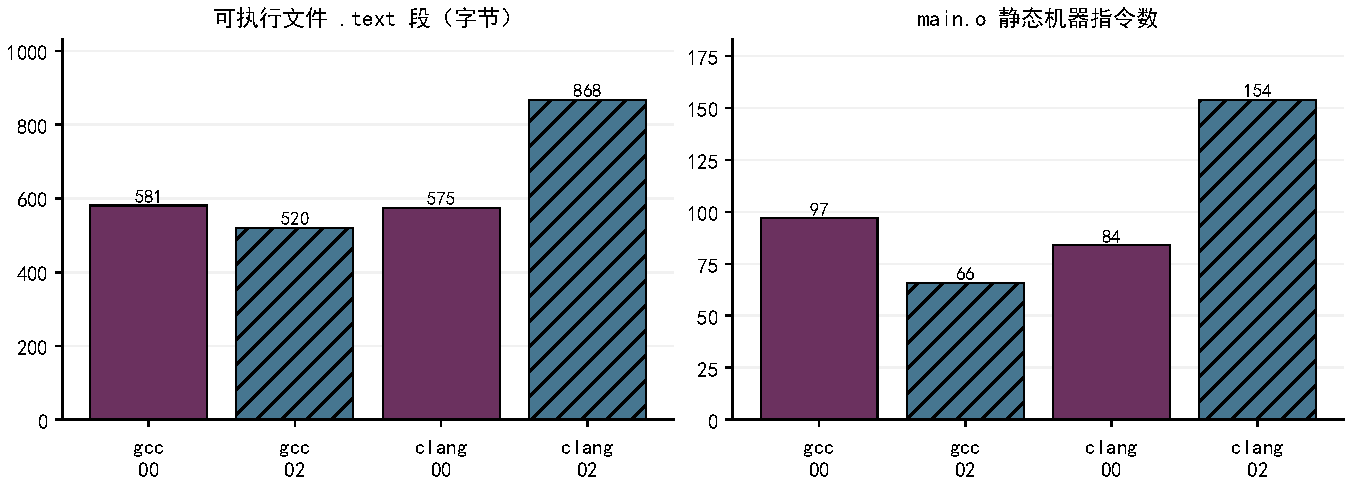
\includegraphics[width=\textwidth]{figures/toolchain_metrics.pdf}
\caption{代码结构指标：左图含链接启动代码，右图只计 \texttt{main.o} 的静态指令行（含填充 nop）。}
\label{fig:metrics}
\end{figure}
Clang O2 的 \texttt{.text} 从 575 B 增至 868 B，静态指令数从 84 增至 154。向量主体、横向归约、入口判断、标量尾部，以及内联后仍保留的独立函数定义都需要空间；\texttt{main} 的有界展开还改变了控制流。这些结构解释了为何优化可能增大代码。本文未进行逐 pass 消融，各结构对代码增量的单独贡献尚未量化。

GCC O2 的对应指标由 581 B/97 条降至 520 B/66 条，其循环改为从 5 开始每轮加 3 的归纳变量，分支变成 \texttt{testb/cmove}。同参数的 \texttt{gcc -Q --help=optimizers} 显示，\texttt{-ftree-loop-vectorize} 和 \texttt{-ftree-slp-vectorize} 均为 \texttt{[disabled]}；GCC 11.4 官方文档也将两者列为 O3 默认开启\cite{gccopt11}。本例的 GCC O2 配置没有启用这两类向量化优化；上述基线未包含 O3；本轮新增比较见\ref{sec:toolchain-gcc-controlled}节。

两者虽均指定通用 x86-64，完整优化流水线没有逐项对齐，GCC 默认安全选项及 O2 的 \texttt{\_FORTIFY\_SOURCE=2} 还改变系统头文件展开，其 O0 和 Clang O2 没有该宏。LLVM 的宽度与交错选择使用代价模型\cite{llvmvector14}；\texttt{main} 的诊断报告“交错无收益”，但没有给出该判断的数值成本。由于 GCC 与 Clang 在 O2 下启用的优化集合不同，代码大小差异不能直接用于评价两种编译器的优劣。本实验未测运行时间，不进行性能比较；文件大小和静态指令数量仅用于描述产物结构，不能据此推断执行时间。

O2 加 \texttt{-g} 后，GCC/Clang 可执行文件分别由 16216/16120 B 增至 21080/19136 B，\texttt{.debug*} 合计为 4239/2315 B。在本例中，两编译器各自 O2 与 O2-g 的整个 \texttt{.text} 内容相同，文件增长还含节表等元数据。跨翻译单元的 \texttt{add\_bonus} 调用仍保留，内联诊断说明其定义不可见；实验没有启用 LTO。

新增实验为上述解释补充了可量化的配置对照：Clang 的空间差异与向量主体、交错、展开及尾部结构共同变化，GCC O3 的差异则在未发生向量化的情况下伴随 \texttt{main} 内联。它们仍不构成逐 pass 的独立消融。诊断构建与普通构建逐一比较目标文件全部可执行代码节，GCC 同时检查 \texttt{.text} 与包含 \texttt{main} 的 \texttt{.text.startup}，九组均保持一致；只检查 GCC 的 \texttt{.text} 会漏掉 \texttt{main}，因此不能据其单节哈希断言整个目标代码相同。原有 60/60、新增配置 90/90 和边界入口 12/12 各自保留统计口径，均未转化为性能结论。

\section{基本要求二：SysY 程序的 LLVM IR 与 RISC-V 等价实现及验证}
\label{sec:sysy}
\subsection{SysY 示例程序设计与语言特性覆盖}
\label{sec:sysy-coverage}
本实验设计两个互补的 SysY 示例，以整数控制逻辑和浮点数据处理分别检验语言特性的实现。先确定源程序的计算语义、有效输入域与独立预期，再分别分析手写 LLVM IR 和 RISC-V 汇编，最后通过运行库集成、目标程序构建与运行测试检查语义一致性。

\subsubsection{示例程序设计与语言特性覆盖}
\label{sec:sysy-example-design}
\texttt{control\_matrix} 检验整数运算、赋值与初始化、条件分支、循环、\texttt{break/continue}、短路副作用、二维数组、函数调用、作用域及有符号除余；\texttt{float\_stats} 检验单精度浮点运算、一维浮点数组、函数调用、整数与浮点混合参数以及类型转换。两个程序各有 SysY 源程序，以及独立手写的 \texttt{.ll/.S} 等价实现，便于对照同一源语义在不同抽象层次中的表达。

表\ref{tab:coverage}将课程要求逐项对应到两个源程序中的构造，并列出 IR 或汇编实现机制。表中的位置以函数、变量或表达式标识，便于将语言特性与后续分析联系起来。
\Needspace{14\baselineskip}
\begingroup
\small
\setlength{\tabcolsep}{5pt}
\begin{longtable}{L{2.35cm}L{6.35cm}L{5.6cm}}
\caption{课程语言特性要求与 SysY 示例覆盖位置}
\label{tab:coverage}\\
\toprule\rowcolor{tableHead}课程要求 & 本实验源码位置 & 对应机制与验证 \\
\midrule
\endfirsthead
\toprule\rowcolor{tableHead}课程要求 & 本实验源码位置 & 对应机制与验证 \\
\midrule
\endhead
\bottomrule
\endfoot
\texttt{int/float} 与变量声明 & \texttt{control\_matrix} 的 \texttt{n/i/sum}；\texttt{float\_stats} 的 \texttt{scale/result} & \texttt{i32/float} 类型；整数与单精度浮点分别运算。\\
常量与初始化 & \texttt{COLS=3}、\texttt{SHIFT=0.25}；整数二维数组与浮点一维数组初值 & \texttt{COLS} 用于行列索引计算，\texttt{SHIFT} 用于结果偏置；二维数组部分初始化补零。\\
数值运算 \texttt{+,-,*} & \texttt{tick} 的一元 \texttt{+x}；\texttt{fold} 的 \texttt{n-1}、\texttt{sum+v*i}；\texttt{affine} 的乘加 & 一元加保持值；\texttt{add/sub/mul} 与 \texttt{fmul/fadd}。\\
数值运算 \texttt{/,\%} & \texttt{cell} 调用参数 \texttt{i/COLS,i\%COLS}；整数输出中的除余；\texttt{normalized} 的浮点除法 & \texttt{sdiv/srem} 与 \texttt{divw/remw}；\texttt{fdiv/fdiv.s}。\\
关系运算 & 整数 \texttt{fold/main} 覆盖 \texttt{<=,<,>,==,!=}；\texttt{sum\_positive} 的整数循环条件使用 \texttt{>=}，浮点筛选使用 \texttt{v>0.0} & 整数 \texttt{icmp}、浮点 \texttt{fcmp} 与条件分支。\\
\texttt{\&\&,||,!} & 整数 \texttt{main} 中两条含 \texttt{tick} 的条件及 \texttt{if(!gate)} & 短路以控制流实现；全局 \texttt{calls} 记录副作用次数。\\
赋值 & \texttt{calls=calls+1}、\texttt{sum=sum+v*i} 与 \texttt{a[i]=getfloat()} & SSA 新值、全局/数组 \texttt{store}；汇编寄存器和内存更新。\\
\texttt{if/while} & \texttt{fold} 的循环与判断；\texttt{sum\_positive} 的正值筛选 & 条件基本块、回边与汇编 branch/label。\\
\texttt{return} & \texttt{tick/cell/fold/affine} 返回值；\texttt{separator} 的无值返回 & LLVM \texttt{ret}；整数/浮点返回使用 \texttt{a0/fa0}。\\
\makecell[l]{\texttt{break}\\\texttt{continue}} & \texttt{fold} 中零值跳过与 stop 提前终止 & \texttt{body}$\to$\texttt{step} 与 \texttt{check.break}$\to$\texttt{exit}；phi 与回边。\\
函数定义与调用 & \texttt{cell/fold/tick}；无参 void 函数 \texttt{separator}；\texttt{affine/sum\_positive} & 带参返回函数与无参 void 函数；\texttt{call} 与 ABI 传参。\\
作用域 & 全局 \texttt{bias=7} 与整数 \texttt{main} 内层块的 \texttt{bias=3} & 名字遮蔽后分别贡献 7 与 3，全局变量值未被局部声明改变。\\
一维/二维数组 & 两个 \texttt{main} 中的 \texttt{float a[4]}、\texttt{int a[2][3]}；\texttt{cell(int a[][3],...)} & 浮点元素 GEP 与行指针 GEP；二维行跨度 12 字节。\\
浮点与混合调用 & \texttt{affine(float x,float scale,int offset)}、\texttt{sum\_positive} & 整数/浮点参数寄存器独立分配；binary32 舍入。\\
类型转换 & \texttt{affine} 将整数 offset 加入浮点乘积；\texttt{int truncated=result} & \texttt{sitofp/fcvt.s.w}；\texttt{fptosi/fcvt.w.s rtz} 向零截断。\\
输入输出与运行库 & \makecell[l]{\texttt{getint/getfloat}\\\texttt{putint/putfloat/putch}} & 静态链接 SysY 运行库，调用目标 glibc。\\
张量类型 & 未覆盖 & 课程材料未提供具体语法与语义定义。\\
\end{longtable}
\endgroup

\subsubsection{\texttt{control\_matrix}：整数运算与控制流}
\label{sec:sysy-integer-semantics}

该程序对更新后的二维整数数组进行带提前终止条件的加权求和，同时输出短路调用次数、条件分支标记和有符号除余结果。\texttt{cell} 按给定行、列返回数组元素；\texttt{fold} 将线性位置分别除以和取余 \texttt{COLS}，据此访问对应元素。

二维部分初始化 \texttt{\{\{1,2\},\{-3,4,5\}\}} 产生 $[1,2,0,-3,4,5]$。输入是 \texttt{n}、\texttt{stop}、\texttt{gate}、\texttt{divisor} 和六个增量；更新后元素记为 $a_i$。\texttt{fold} 检查前 $n$ 个位置，先递增索引，遇 0 执行 continue，遇非零 stop 执行 break，其余贡献 $(i+1)a_i$；第一项输出再加全局 7 与局部 3。因此 stop=0 不会把零元素当作停止点。

其余输出为 \texttt{calls,tag,q,r}。gate=0 时 \texttt{\&\&} 的 RHS 和 \texttt{||} 已为真的左侧之后的 RHS 均跳过，故 \texttt{calls=0,tag=6}；gate 非零且首元素正、末元素负时，两次 tick 均执行，得到 \texttt{calls=2,tag=3}。SysY 将 \texttt{Exp} 与 \texttt{Cond} 分开，括号基本表达式只包围 \texttt{Exp}；源码中的布尔条件依赖 \texttt{\&\&} 高于 \texttt{||} 的优先级组织，符合这一文法约束。

\texttt{calls} 记录 \texttt{tick} 对全局状态的修改次数，\texttt{tag} 记录三条条件语句的分支结果；\texttt{q,r} 分别是更新后 \texttt{a[0][1]} 除以 \texttt{divisor} 的商与余数。内层块中的 \texttt{bias=3} 遮蔽全局名字，只将 3 赋给 \texttt{local}，不改变全局 \texttt{bias=7}，两者在第一项输出中分别贡献偏置。

有效域为 $0\le n\le6$、增量 $[-30,30]$、stop $[-40,40]$、gate $[-2,2]$，divisor 为 $[-7,7]$ 内非零数，保证无越界、溢出、除零及 \texttt{INT\_MIN/-1}。oracle 直接计算首个非零 stop 之前的加权前缀和；商以绝对值整除后补符号，余数用 $r=a-qd$，避免误用 Python 对负数向下取整的语义。

\subsubsection{\texttt{float\_stats}：浮点运算与函数调用}
\label{sec:sysy-float-semantics}
\texttt{float\_stats} 对一维数组元素进行仿射变换，筛选正值并累加，再输出带偏置的结果及其两种派生值。程序输入为整数 \texttt{n}、单精度 \texttt{scale} 和 \texttt{n} 个浮点元素。\texttt{float a[4]} 初值为 $[1.0,-2.0,0.5,0.0]$，输入覆盖前 \texttt{n} 项，未参与计算的其余元素不影响结果。

\texttt{affine(float x,float scale,int offset)} 计算 \texttt{x*scale+offset}，其中整数 \texttt{offset} 转为浮点后参与加法。\texttt{sum\_positive} 从 \texttt{i=0,sum=0.0} 开始，在整数条件 \texttt{n>=i+1} 成立时调用 \texttt{affine(a[i],scale,i)}；仅当返回值 \texttt{v>0.0} 时将其加入累计和，然后递增索引。该设计同时覆盖浮点函数返回值、混合类型参数、正值筛选和有序累加。

\Needspace{10\baselineskip}
源程序的预期必须包含单精度舍入，而非仅按实数计算最终公式。记 $\operatorname{fl}_{32}$ 为独立数值 oracle 使用的 binary32 舍入，输入的 \texttt{a} 和 \texttt{scale} 已转换为 binary32。第 $i$ 项及累计状态为
\begin{equation}
\begin{aligned}
p_i&=\operatorname{fl}_{32}(a_i\,scale),&
v_i&=\operatorname{fl}_{32}\bigl(p_i+\operatorname{fl}_{32}(i)\bigr),\\
S_0&=0,&
S_{i+1}&=
\begin{cases}
\operatorname{fl}_{32}(S_i+v_i),&v_i>0,\\
S_i,&v_i\le0.
\end{cases}
\end{aligned}
\label{eq:sysy-float-oracle}
\end{equation}
乘法、仿射加法与每次累加分别舍入，不将乘加合并为一次运算。随后 \texttt{result} 为累计和加 0.25 后的 binary32 结果，\texttt{truncated} 为 \texttt{result} 向零截断得到的整数；\texttt{normalized} 将同一 \texttt{result} 除以整数 $n+1$ 转换后的浮点值，并再次舍入。程序按 \texttt{result,truncated,normalized} 的顺序输出，以空格分隔、换行结束。这里的 \texttt{normalized} 分母为 \texttt{n+1}，分子包含正值筛选与偏置，表示程序定义的归一化结果。

有效域为 $0\le n\le4$、有限数、$|scale|\le8,|a_i|\le32$；oracle 每步舍入至 binary32，浮点误差要求 $|y-\widehat y|\le10^{-6}+2\times10^{-6}|\widehat y|$，整数精确比较，不扩展到 NaN/Inf、次正规数或越界转换。\texttt{tests/sysy\_oracle.py} 使用 \texttt{struct} 的单精度打包与解包构造独立预期，明确区分乘、加、筛选、累加、偏置、向零转换和除法的先后次序。上述计算定义及独立预期是后续分析两种底层实现的依据。

\subsection{LLVM IR 等价实现与关键语义映射}
\label{sec:sysy-ir}
LLVM IR 用类型化指令表达运算，用基本块和分支表达控制流，用 SSA 值及 phi 节点表达变量更新。数组和全局变量仍通过内存访问实现。等价实现要求保留源程序的求值顺序、数据布局和副作用。

\subsubsection{基本块与条件控制流}
\label{sec:sysy-ir-blocks}
SysY 的 \texttt{if} 与 \texttt{while} 条件对应 LLVM 的比较指令和 \texttt{br}。例如 \texttt{fold} 的 \texttt{icmp sle} 决定进入循环体还是退出；\texttt{tick} 对全局变量的赋值则由 \texttt{load/add/store} 表达。为同时观察循环路径与短路路径，图\ref{fig:llvm-fold-cfg}分别展示 \texttt{fold} 与 \texttt{main} 的控制流。

图\ref{fig:llvm-fold-cfg}根据手写 IR 的终结指令绘制：\texttt{fold} 有七个块、九条边，\texttt{continue} 与 \texttt{break} 分别对应到 \texttt{step} 和 \texttt{exit} 的控制流边。该 IR 通过 \texttt{opt-14 -verify} 验证，其支配关系由 dominator-tree 分析得到。

\begin{figure}[H]
\centering
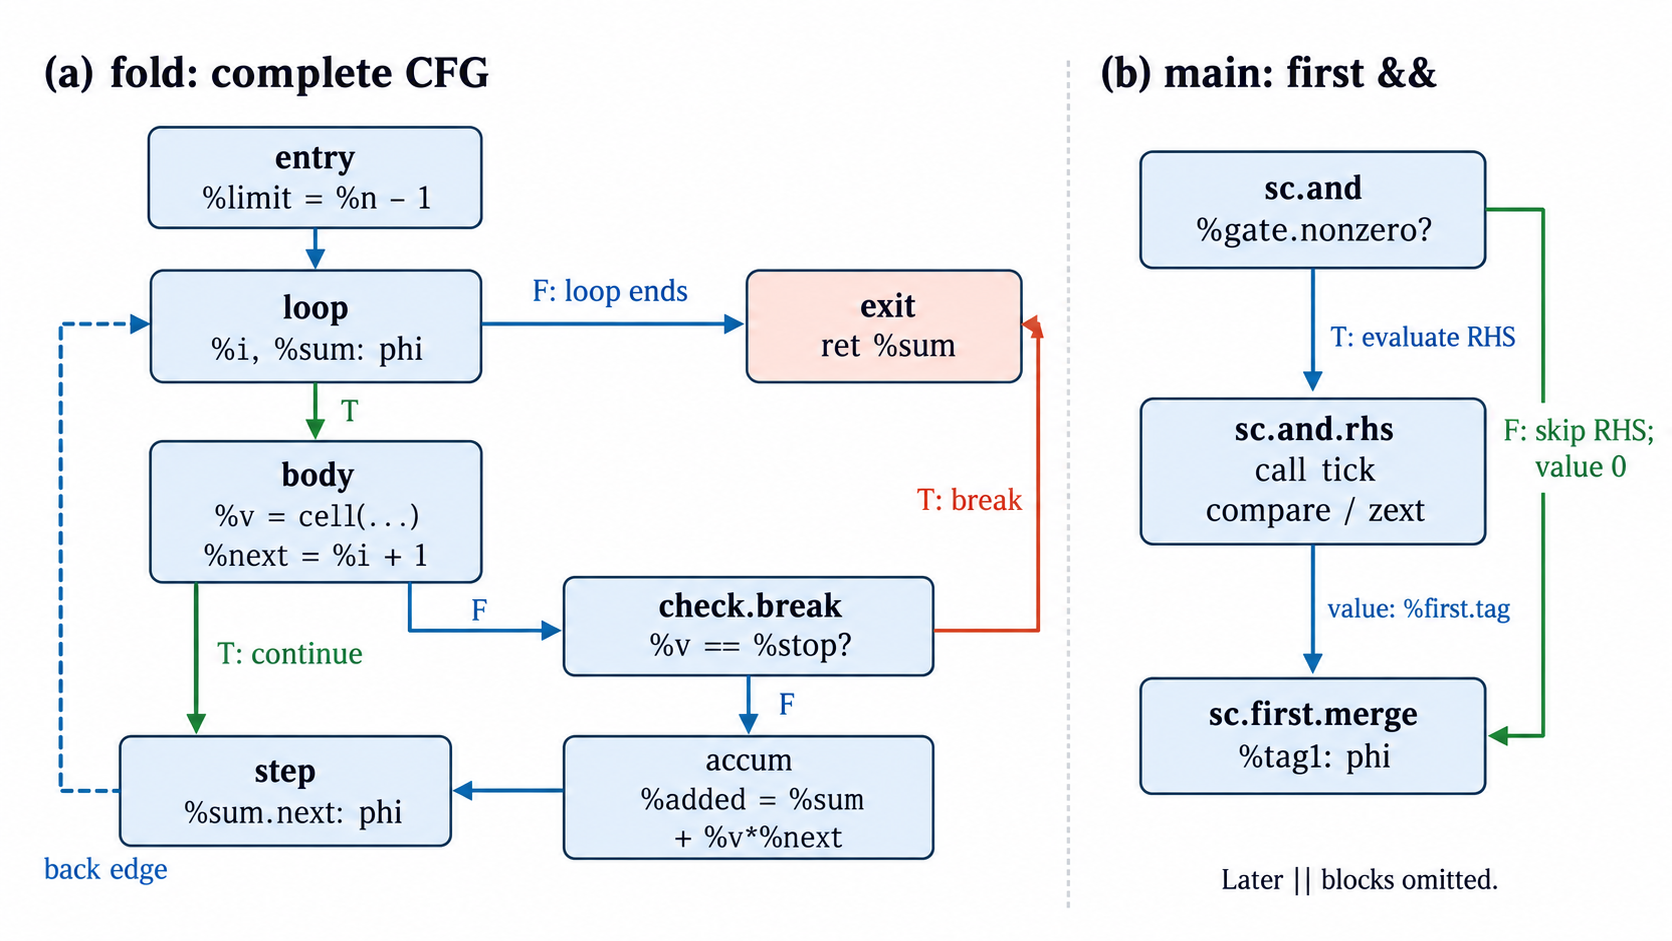
\includegraphics[width=\textwidth,keepaspectratio]{figures/fig3.png}
\caption{LLVM IR 控制流图。（a）\texttt{fold} 函数的完整 CFG，虚线表示循环回边；body 的 T/F 分别对应 \texttt{v==0} 的真假分支，continue 与 break 分别跳转至 \texttt{step} 和 \texttt{exit}。（b）\texttt{main} 中首个 \texttt{\&\&} 的短路求值子图，左操作数为假时跳过 \texttt{tick} 调用，为真时执行右操作数，并在 phi 节点合并结果。后续 \texttt{||} 相关基本块未展示。}
\label{fig:llvm-fold-cfg}
\end{figure}

\subsubsection{循环、break 与 continue}
\label{sec:sysy-ir-loops}
\texttt{while} 的循环条件位于 \texttt{loop}，循环体完成后经 \texttt{step} 回到条件块；索引已在 \texttt{body} 中、判断 \texttt{continue} 之前递增。\texttt{continue} 保留已有累计和并经 \texttt{step} 回跳，\texttt{break} 则直接到达退出块。表\ref{tab:source-cfg-ssa}按源语句对应其控制流边与 SSA 状态，说明每条跳转保留了哪一项源语义。

\begin{table}[H]
\centering\small
\caption{选取 \texttt{fold} 的关键源语句，逐项映射到 CFG 与 SSA}
\label{tab:source-cfg-ssa}
\begin{tabularx}{\textwidth}{L{4.45cm}L{3.0cm}Y}
\toprule\rowcolor{tableHead}SysY 源构造 & CFG 位置/边 & LLVM IR 状态 \\
\midrule
\texttt{int i=0,sum=0;} & \texttt{entry}$\to$\texttt{loop} & 两条 phi 的初次来值均为 0。\\
\texttt{while(i<=n-1)} & \texttt{loop} 条件及回边 & \texttt{icmp sle}；\texttt{\%i/\%sum} 为当前迭代状态。\\
\texttt{v=cell(...); i=i+1;} & \texttt{body} & 调用结果 \texttt{\%v}；递增值 \texttt{\%next}。\\
\texttt{if(v==0) continue;} & \texttt{body}$\to$\texttt{step} & 保留 \texttt{\%sum}，索引仍推进。\\
\texttt{if(v==stop) break;} & \makecell[l]{\texttt{check.break}\\$\to$\texttt{exit}} & 跳过累加与回边，返回当前 \texttt{\%sum}。\\
\texttt{sum=sum+v*i;} & \texttt{accum}$\to$\texttt{step} & 新值 \texttt{\%added} 进入 \texttt{\%sum.next}。\\
\texttt{return sum;} & \texttt{exit} & \texttt{ret i32 \%sum}，没有额外 exit phi。\\
\bottomrule
\end{tabularx}
\end{table}

\subsubsection{SSA 与 phi：变量赋值、前驱和支配关系}
\label{sec:sysy-ir-ssa}
源程序对 \texttt{i/sum} 的重复赋值，在 SSA 中分别产生新的值。循环入口与回边、正常累加与 continue 路径会带来不同值，phi 必须根据进入基本块的前驱边选择，才能实现对应的变量状态。

phi 的 incoming pair 是“值、前驱块”而非“条件、候选值”，其使用点视为对应入边\cite{llvm}。本例三个 phi 的关系如下：
\begin{enumerate}[itemsep=0.1em,topsep=0.1em]
\item \texttt{\%i = phi i32 [0,\%entry],[\%next,\%step]}：首次从 entry 取 0；以后从 step 取 body 已算好的 next。body 支配 step，故 continue 和累加两条到达 step 的路径都已定义 next。
\item \texttt{\%sum = phi i32 [0,\%entry],[\%sum.next,\%step]}：入口值为 0；每次回边取 step 内先行定义的 sum.next，而非不加区分地取 added。
\item \texttt{\%sum.next = phi i32 [\%sum,\%body],[\%added,\%accum]}：

body 入边是 continue，取旧 sum；accum 入边取刚定义的 added。added 无须支配整个 step，只需在 \texttt{accum}$\to$\texttt{step} 边上可用。
\end{enumerate}

dominator tree 显示 loop 支配 body 与 exit、body 支配 step。accum 不支配 step，其值在此合流，体现支配边界与 phi 放置的关系。源变量 sum 在 SSA 中对应 sum、added、sum.next 多个值。break 必须绕过 step：若错误地走 step 回边，就继续下一轮而没有终止。正常退出由 loop、break 退出由 check.break 到达 exit，两条路径上的 \texttt{\%sum} 均已定义，所以 exit 直接使用它：前者是全部已完成轮次之和，后者不含 stop 元素；$n=0$ 时就是入口 0。

\subsubsection{短路求值与副作用保持}
\label{sec:sysy-ir-short-circuit}
\texttt{\&\&} 与 \texttt{||} 的语义包含是否执行右操作数，不能只比较最终真假值。图\ref{fig:llvm-fold-cfg}右侧的子图用于解释 \texttt{gate != 0 \&\& tick(...)} 中调用的执行条件。

图中控制判断先决定是否进入 \texttt{sc.and.rhs}，tick 的全局写入只发生在真边上；假边直接进入 merge，并为 tag1 提供 0。若写成先 \texttt{call tick} 后 \texttt{select condition}，副作用在选择之前已经发生，select 只能选值，不能撤销写入。因此短路是执行路径的约束，不只是布尔值公式的等价；这里的先后关系是单线程语义顺序，不是硬件内存屏障。

手写 IR 中，上述判断位于 \texttt{sc.and}；真边进入 \texttt{sc.and.rhs} 执行调用，假边绕过调用，两条路径在 \texttt{sc.first.merge} 由 phi 合并 \texttt{tag1}。后续 \texttt{||} 及其右侧嵌套的 \texttt{\&\&} 同样通过条件分支控制调用是否发生，保留前述 \texttt{calls} 与 \texttt{tag} 的源语义。

\subsubsection{二维数组与 GEP 寻址}
\label{sec:sysy-ir-gep}
数组读写的等价性要求索引顺序、元素类型和行跨度一致；本例用 GEP 的类型结构表达二维数组的连续布局。

数组寻址也保留类型信息：main 的 \texttt{[2 x [3 x i32]]} GEP 先取对象层 0，再取行列；cell 接收 \texttt{[3 x i32]*}，行步长为 $3\times4=12$ 字节。\texttt{sext i32 to i64} 后形成 $\operatorname{base}+4(3r+c)$；行跨度由数组元素类型决定，与 8 字节指针宽度无关。此处二维数组的元素连续存储，其布局区别于指针数组。

\subsubsection{浮点运算与类型转换}
\label{sec:sysy-ir-float}
\texttt{float\_stats.ll} 使用 LLVM \texttt{float} 类型表达前述单精度计算，将浮点算术、整数循环条件与浮点筛选分别表示，保留源程序的运算顺序和转换位置。

\texttt{affine} 依次执行 \texttt{fmul float}、\texttt{sitofp i32 \%offset to float} 和 \texttt{fadd float}，对应先乘法、再将整数参数转换为浮点、最后相加。\texttt{sum\_positive} 的循环条件用 \texttt{icmp sge i32} 比较整数 \texttt{n} 与 \texttt{i+1}；\texttt{fcmp ogt float \%v,0.0} 则判断仿射结果是否为正，并以 \texttt{br} 选择累加或跳过。循环入口的 \texttt{phi i32/phi float} 保存索引与累计状态，\texttt{step} 中的 \texttt{phi float} 合并旧累计和与 \texttt{fadd} 产生的新值。

\texttt{main} 先用 \texttt{fadd} 加入 0.25，再以 \texttt{fptosi float \%result to i32} 表达向零截断；分母先由 \texttt{add i32} 计算 \texttt{n+1}，经 \texttt{sitofp} 转为 \texttt{float}，最后执行 \texttt{fdiv}。IR 未使用 \texttt{fast/contract} 标志，乘法与加法保持为分离操作，与式\eqref{eq:sysy-float-oracle}中的逐步舍入定义对应。转换与比较的等价性限定在前述有效输入域内，不据此扩展到越界转换或特殊浮点值。

\addtocontents{toc}{\protect\Needspace{4em}}
\subsection{RISC-V 汇编等价实现与底层机制}
\label{sec:sysy-riscv}
RISC-V 实现面向 RV64GC 指令集，用机器指令完成数值运算，用 branch/label 组织控制流，并按 LP64D ABI 传递参数、保存活跃值和返回结果。下面分别对应 SysY 的运算、控制和函数调用语义。

\subsubsection{整数运算与 RISC-V 指令映射}
\label{sec:sysy-riscv-integer}

RV64 的寄存器/地址为64位，但 SysY int 的存储和运算仍为32位。整数程序的 lw 读4字节再符号扩展，sw 只写低32位；addw、mulw 形成32位结果后符号扩展，divw/remw 对低32位做有符号除余。循环递减界限采用 \texttt{addiw ..., -1}\cite{riscv-isa}。替换成64位 long 运算会改变位宽截断约束；数组基址相加则使用完整64位 add，以保留地址位宽。实验输入已排除有符号溢出。

\subsubsection{条件分支与循环控制}
\label{sec:sysy-riscv-branches}
整数 \texttt{fold} 在 \texttt{.Lfold\_loop} 用 \texttt{bgt s3,s1,.Lfold\_exit} 判断循环结束；\texttt{call cell} 后先执行 \texttt{addiw s3,s3,1} 递增索引。随后 \texttt{beqz s5,.Lfold\_loop} 实现 continue，\texttt{beq s5,s2,.Lfold\_exit} 实现 break；其顺序保证 stop=0 时先跳过零元素。正常累加由 \texttt{mulw/addw} 完成，再用 \texttt{j .Lfold\_loop} 形成回边。

整数 \texttt{main} 的 \texttt{beqz s2,.Lsc\_or} 在 gate=0 时跳过第一个 \texttt{tick}；到达 \texttt{.Lsc\_or} 后，\texttt{beqz s2,.Lsc\_add2} 跳过 \texttt{||} 右侧。\texttt{bgez a0,.Lsc\_not} 决定嵌套 \texttt{\&\&} 是否调用 \texttt{tick}，\texttt{bnez s2,.Lcompute} 实现 \texttt{!gate} 的真假选择。浮点循环在 \texttt{.Lfloat\_loop} 用 \texttt{blt s1,t0,.Lfloat\_exit} 实现 \texttt{n>=i+1}；\texttt{flt.s} 的结果经 \texttt{beqz} 决定是否累加，随后在 \texttt{.Lfloat\_step} 递增索引并回跳。

\subsubsection{函数参数传递与调用约定}
\label{sec:sysy-riscv-parameters}
整数函数 \texttt{fold} 的数组地址、n 和 stop 分别放在 \texttt{a0/a1/a2}。\texttt{sum\_positive} 的数组地址和 n 使用 \texttt{a0/a1}，scale 作为第一个浮点参数使用 \texttt{fa0}；整数参数与浮点参数按各自的寄存器序列分配。

\texttt{float\_stats.S} 中 \texttt{affine} 是仅有乘法、转换、加法和 ret 的叶函数，没有栈帧。图\ref{fig:riscv-call-frame}将汇编指令与 LP64D 参数分配对照：x 与 scale 分别使用 \texttt{fa0/fa1}；整数和浮点参数寄存器独立分配，因此第三个源参数 offset 使用 a0，而不是 a2；float 返回复用 fa0\cite{riscvabi}。

\subsubsection{寄存器保存与函数调用}
\label{sec:sysy-riscv-save}
函数调用可能改写 caller-saved 寄存器，跨调用仍需使用的状态必须由调用方保护；使用 callee-saved 寄存器的函数则负责保存并恢复调用者的值。\texttt{sum\_positive} 调用 \texttt{affine}，可用于观察这两类责任。

在 \texttt{call affine} 前，后续仍需要数组地址、n、i、scale 与累计 sum，分别保留在 \texttt{s0/s1/s2/fs0/fs1}。当前元素 x 已装入 fa0，scale 从 fs0 复制到 fa1，i 从 s2 复制到 a0；返回后 fa0 改为仿射结果 v。计算元素地址的 t0 此时已无后续用途，而 affine 会改写 ft0。这些 caller-saved 临时寄存器的值不受被调用者保护，因此本实现将跨调用的活跃值保存在 callee-saved 寄存器中。

\subsubsection{栈帧组织与数据保护}
\label{sec:sysy-riscv-frame}
图\ref{fig:riscv-call-frame}对照叶函数的参数映射与非叶函数的保存区：\texttt{affine} 不建立栈帧，\texttt{sum\_positive} 使用 64 字节栈帧保存返回地址和寄存器。图中的偏移对应其入口保存和出口恢复指令。

以减去 64 后的新 \texttt{sp} 为基准，保存槽依次为 \texttt{fs1:16(sp)}、\texttt{fs0:24(sp)}、\texttt{s2:32(sp)}、\texttt{s1:40(sp)}、\texttt{s0:48(sp)} 和 \texttt{ra:56(sp)}；各槽占 8 字节，0--15 字节未使用。它们与 \texttt{float\_stats.S} 的保存、恢复指令逐项对应。

\begin{figure}[H]
\centering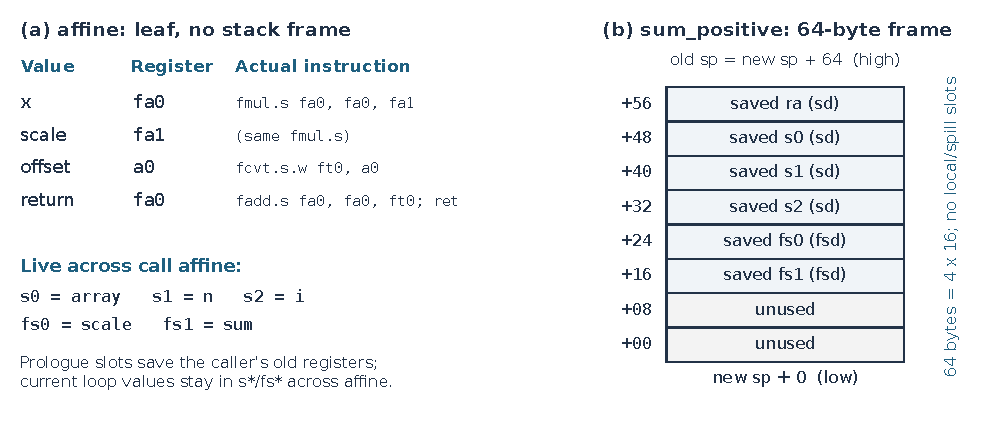
\includegraphics[width=\textwidth]{figures/riscv-call-frame.pdf}
\caption{左：\texttt{affine} 的参数映射，该叶函数不建立栈帧；右：\texttt{sum\_positive} 的非叶栈帧。偏移以减去 64 后的新 sp 为基准，每格 8 字节；0--15 字节未使用，没有局部数组或 spill 槽。}
\label{fig:riscv-call-frame}
\end{figure}

\Needspace{4\baselineskip}
要区分两种保护：当前循环状态跨 affine 调用留在 s/fs 寄存器中，该叶函数确实不修改它们；栈上保存的则是进入 sum\_positive 时\emph{调用者原来的} s/fs 值，并非每轮当前 sum 的副本。call 改写 ra，故入口将原返回地址存于 \texttt{56(sp)}。退出时先把当前 fs1 复制到 fa0，再依次恢复 fs1/fs0/s2/s1/s0/ra，最后加回 64 并 ret。$64=4\times16$ 保持栈对齐，fsd/fld 保存完整64位寄存器状态。

\subsubsection{浮点运算与类型转换}
\label{sec:sysy-riscv-float}
浮点等价实现需要保持单精度运算的舍入位置，并使浮点到整数的转换采用 SysY 所要求的向零截断。

浮点乘加使用 \texttt{fmul.s/fadd.s} 两次舍入，无融合乘加；整数 offset 用 \texttt{fcvt.s.w}，最终 \texttt{fcvt.w.s ...,rtz} 与 IR 的 \texttt{fptosi} 对应向零截断。这里保留的是\hyperref[sec:sysy-float-semantics]{浮点示例计算定义}中的各个舍入位置：\texttt{affine} 不使用 \texttt{fmadd.s}，正值累计和结果偏置分别使用独立的 \texttt{fadd.s}；分母经 \texttt{addiw} 和 \texttt{fcvt.s.w} 后，\texttt{fdiv.s} 产生最后一项输出。数组元素通过 \texttt{flw/fsw} 按 4 字节访问，与保存浮点寄存器状态的 \texttt{fsd/fld} 用途不同。源程序计算过程、有效域与 oracle 已在示例设计部分定义，这里据此核对机器指令的位宽、转换模式和运算顺序。

\subsubsection{LLVM IR 与 RISC-V 的语义映射对照}
\label{sec:sysy-semantic-mapping}
表\ref{tab:sysy-semantic-mapping}归纳两种手写实现对同一 SysY 语义的表达。各项机制均对应当前 \texttt{control\_matrix} 或 \texttt{float\_stats} 的手写 IR 与汇编文件中的实际操作。

\begingroup
\small
\setlength{\tabcolsep}{4pt}
\begin{longtable}{L{2.0cm}L{4.0cm}L{4.0cm}L{4.5cm}}
\caption{SysY 语言特性在 LLVM IR 与 RISC-V 汇编中的实现对应关系}
\label{tab:sysy-semantic-mapping}\\
\toprule\rowcolor{tableHead}SysY 语义 & LLVM IR 关键机制 & RISC-V 关键机制 & 语义保持要点 \\
\midrule
\endfirsthead
\toprule\rowcolor{tableHead}SysY 语义 & LLVM IR 关键机制 & RISC-V 关键机制 & 语义保持要点 \\
\midrule
\endhead
\bottomrule
\endfoot
整数运算 & \texttt{add/mul i32}、\texttt{sdiv/srem} & \texttt{addw/mulw}、\texttt{divw/remw} & 保持 32 位整数结果及有符号除余行为。\\
条件分支 & 整数 \texttt{icmp/br}；浮点 \texttt{fcmp ogt/br} & \texttt{bgt/beqz/beq} 等分支；\texttt{flt.s} 后分支 & 比较对象、真假方向及执行路径一致。\\
循环 & \texttt{loop/body/step/exit} 基本块与回边 & 循环标签、\texttt{addiw} 与 \texttt{j} 回跳 & 保持迭代边界、索引递增及提前终止。\\
变量更新 & \texttt{phi} 合并 SSA 值；\texttt{load/add/store} 更新全局状态 & 寄存器更新；\texttt{lw/addiw/sw} 更新 \texttt{calls} & 按实际前驱路径选择状态并保留可观察写入。\\
短路求值 & 条件 \texttt{br} 决定 \texttt{call tick} 是否执行，phi 合流 & \texttt{beqz/bgez} 等跳转绕过或进入调用 & RHS 的全局副作用仅在源语义要求的路径发生。\\
数组访问 & 类型化 \texttt{getelementptr}，元素 \texttt{load/store} & 行列偏移、\texttt{slli/add}，整数 \texttt{lw/sw}、浮点 \texttt{flw/fsw} & 二维行跨度 12 字节，整数和浮点元素均占 4 字节。\\
函数调用 & 带类型的 \texttt{call/ret} 及参数、返回值 & LP64D 的 \texttt{a/fa} 参数与返回寄存器，\texttt{call/ret} 及保存恢复 & 参数类别、顺序、返回值和跨调用活跃状态一致。\\
浮点运算 & \texttt{float} 上的 \texttt{fmul/fadd/fdiv} & \texttt{fmul.s/fadd.s}、\texttt{fdiv.s} & 保持 binary32 运算顺序和分离乘加的舍入位置。\\
类型转换 & \texttt{sitofp} 与 \texttt{fptosi} & \texttt{fcvt.s.w} 与 \texttt{fcvt.w.s ...,rtz} & 整数到单精度转换；浮点到整数向零截断。\\
\end{longtable}
\endgroup

同一 SysY 语义在 LLVM IR 中主要通过类型化操作、控制流和 SSA 表达，在 RISC-V 中则由机器指令、寄存器状态及 ABI 约束共同实现。表中的对应关系属于语义层面的归纳，并非指令严格一一对应；循环、短路与函数调用通常需要多个基本块或多条机器指令协作。下面将两种独立实现与源程序基准统一接入运行库，再分别构建并验证。

\subsection{SysY 运行时库的构建与集成}
\label{sec:sysy-runtime}
输入输出函数由链接的 SysY 运行库提供；程序只调用相应接口，目标 glibc 承担底层输入输出。运行库编译为目标对象并归档为 \texttt{libsylib.a}，再参与各程序的最终静态链接。
实验参考 SysY2022 语言定义与运行库说明\cite{sysyspec}。由于课程专用运行库原件未提供，本实验采用公开的 SysY2022 兼容实现\cite{runtime}；\texttt{getint/getfloat/putint/putfloat/putch} 由该运行库提供，并调用目标 glibc。

运行库的构建命令如下，目标架构与三个程序路径均为 RV64GC/LP64D：
\begin{lstlisting}[caption={SysY 运行库对象与静态归档的构建},label={lst:sysy-runtime-build}]
riscv64-linux-gnu-gcc -std=c11 -O2 -fcommon -march=rv64gc -mabi=lp64d -c runtime/sylib.c -o artifacts/sysy/objects/sylib.o
riscv64-linux-gnu-ar rcs artifacts/sysy/objects/libsylib.a artifacts/sysy/objects/sylib.o
\end{lstlisting}
运行库头文件含全局暂定定义，使用 \texttt{-fcommon} 兼容其定义方式。链接 map 显示 \texttt{sylib.o} 满足 getint 等引用。运行库 stderr 的 \texttt{TOTAL: 0H-0M-0S-0us} 表示未启用计时接口时的累计时间，不用于性能分析。

\subsection{三种程序实现的编译与链接}
\label{sec:sysy-build}
本节将源程序基准、手写 LLVM IR 和手写 RISC-V 汇编分别编译为目标对象，并链接为独立的 RISC-V ELF 程序。源实现由 Clang 以 \texttt{-x c} 按 C 兼容子集处理 \texttt{.sy} 文件，通过 \texttt{-include runtime/sylib.h} 注入运行库声明；这一构建基准不等同于自行实现完整 SysY 编译器。LLVM 14 有类型指针 IR 与 RV64GC/LP64D 汇编分别构建。自动生成的 IR 与汇编仅用于结果对照。手写 IR 经验证后由 llc 生成目标文件，手写汇编独立汇编，二者均按 SysY 源语义编写，互不作为对方的自动生成结果。两个示例的六个程序均静态链接 \texttt{libsylib.a} 和目标 glibc，以 \texttt{qemu-riscv64} 执行。目标对象的 ELF 记录显示 RISC-V、RVC、double-float ABI 标志。

图\ref{fig:sysy-build-paths}显示源程序、手写 IR 与手写汇编三条构建路径。由 SysY 到手写 IR/汇编的虚线表示按源语义编写等价实现；后续实线表示工具处理。每条路径分别链接生成一个 ELF 程序，再使用相同输入比较输出。
\begin{figure}[H]
\centering
\begin{tikzpicture}[
  sysybox/.style={draw=blueGray,rounded corners=2pt,fill=softBlue,align=center,text width=3.85cm,minimum height=1.08cm,font=\small},
  sysywide/.style={sysybox,text width=6.6cm},
  buildarrow/.style={-{Stealth[length=2mm]},thick,draw=blueGray},
  writearrow/.style={buildarrow,dashed}
]
\node[sysywide] (meaning) at (0,0) {SysY 示例程序与语义};
\node[sysybox] (source) at (-4.7,-1.75) {SysY 源实现 \texttt{.sy}\\Clang 14 交叉编译};
\node[sysybox] (ir) at (0,-1.75) {手写 LLVM IR \texttt{.ll}\\\texttt{llvm-as / opt / llc}};
\node[sysybox] (asm) at (4.7,-1.75) {手写 RISC-V \texttt{.S}\\交叉 GCC 调用汇编器};
\node[sysybox] (so) at (-4.7,-3.35) {\texttt{source.o}};
\node[sysybox] (io) at (0,-3.35) {\texttt{llvm.o}};
\node[sysybox] (ao) at (4.7,-3.35) {\texttt{asm.o}};
\node[sysywide] (link) at (0,-5.05) {各路径分别静态链接\\\texttt{libsylib.a + glibc}};
\node[sysywide] (elf) at (0,-6.55) {三种 RISC-V ELF 程序};
\node[sysywide] (qemu) at (0,-8.05) {\texttt{qemu-riscv64}：相同输入与输出比较};
\draw[buildarrow] (meaning.south west) -- (source.north);
\draw[writearrow] (meaning.south) -- (ir.north);
\draw[writearrow] (meaning.south east) -- (asm.north);
\draw[buildarrow] (source) -- (so);
\draw[buildarrow] (ir) -- (io);
\draw[buildarrow] (asm) -- (ao);
\draw[buildarrow] (so.south) -- (link.north west);
\draw[buildarrow] (io.south) -- (link.north);
\draw[buildarrow] (ao.south) -- (link.north east);
\draw[buildarrow] (link) -- (elf);
\draw[buildarrow] (elf) -- (qemu);
\end{tikzpicture}
\caption{SysY、手写 LLVM IR 与手写 RISC-V 汇编的三条构建路径。虚线表示按语义手写，实线表示构建与执行；三种实现分别生成可执行程序。}
\label{fig:sysy-build-paths}
\end{figure}

以下以 \texttt{control\_matrix} 为例列出构建命令；\texttt{float\_stats} 使用同一脚本和选项，仅替换程序名。
\begin{lstlisting}[caption={源程序、手写 IR 与手写汇编分别生成目标文件},label={lst:sysy-object-build}]
clang-14 --target=riscv64-linux-gnu --gcc-toolchain=/usr -march=rv64gc -mabi=lp64d -std=c11 -fcommon -ffp-contract=off -O0 -x c -include runtime/sylib.h -c src/sysy/control_matrix.sy -o artifacts/sysy/objects/control_matrix.source.o
llvm-as-14 src/llvm/control_matrix.ll -o artifacts/sysy/objects/control_matrix.bc
opt-14 -verify -disable-output artifacts/sysy/objects/control_matrix.bc
llc-14 -O0 -mtriple=riscv64-linux-gnu -mattr=+m,+a,+f,+d,+c -target-abi=lp64d -filetype=obj artifacts/sysy/objects/control_matrix.bc -o artifacts/sysy/objects/control_matrix.llvm.o
riscv64-linux-gnu-gcc -march=rv64gc -mabi=lp64d -c src/riscv/control_matrix.S -o artifacts/sysy/objects/control_matrix.asm.o
\end{lstlisting}
\texttt{llvm-as-14} 将 IR 文本解析为 bitcode，\texttt{opt-14 -verify} 检查结构合法性，\texttt{llc-14 -filetype=obj} 直接生成目标对象。\texttt{riscv64-linux-gnu-gcc -c} 对 \texttt{.S} 文件调用汇编器，保留独立手写汇编路径。源程序的 \texttt{-ffp-contract=off} 关闭乘加融合，与手写 IR 和汇编的分离乘加一致。

\noindent\begin{minipage}{\linewidth}
下列命令链接 IR 路径；源实现和汇编实现分别替换为 \texttt{source.o} 与 \texttt{asm.o}。运行时由测试程序将输入送入标准输入，并比较标准输出与退出状态。
\begin{lstlisting}[caption={IR 路径的静态链接与执行工具},label={lst:sysy-link-run}]
riscv64-linux-gnu-gcc -static -no-pie -march=rv64gc -mabi=lp64d artifacts/sysy/objects/control_matrix.llvm.o artifacts/sysy/objects/libsylib.a -Wl,-Map,artifacts/sysy/control_matrix.llvm.map -o artifacts/sysy/bin/control_matrix.llvm
qemu-riscv64 artifacts/sysy/bin/control_matrix.llvm
\end{lstlisting}
\end{minipage}

三条路径分别生成可执行程序后，还需在相同输入下与独立预期逐一比较。仅让三份程序相互比较无法排除共同实现错误，因而下面同时检验输出、退出状态和针对特定语义风险的负对照。

\subsection{运行结果与语义一致性验证}
\label{sec:sysy-results}
本节依据两个示例的源语义检验三种独立实现，依次说明测试设计、实际运行结果、注错负对照和验证范围，以区分结构合法、正常退出与语义正确这几种不同条件。

\subsubsection{测试用例与独立预期}
\label{sec:sysy-test-design}
三种实现使用同一组测试输入，并分别与独立数学 oracle 的预期输出比较，同时检查程序退出状态。整数用例限定在前述有效域，排除数组越界、整数溢出和除零；浮点 oracle 按 binary32 逐步舍入，结果按正文给出的绝对/相对组合容差判断，整数输出精确比较。

整数测试包括 20 个固定用例与 80 个按固定种子生成的用例，覆盖空循环、不同停止位置、零值跳过、短路分支、正负除余与增量边界。浮点测试包括 10 个固定用例与 50 个生成用例，覆盖空输入、零或负 scale、正负值筛选、非整数结果与输入边界。生成器先将浮点输入舍入为 binary32，再以十六进制浮点形式送入运行库，减少十进制文本转换歧义。

预期输出独立于三种实现计算：整数采用前述加权前缀和与显式符号除余定义，浮点采用式\eqref{eq:sysy-float-oracle}的逐步舍入过程，再计算偏置、截断与归一化结果；五个手算锚点用于核对 oracle 本身。每次执行保存输入、预期、标准输出、标准错误和退出码，只有退出 0 且输出满足判据才计为通过。浮点输出按数值解析比较，而非字符串逐字比较；容差适用于两个浮点输出，中间的整数输出仍要求精确相同。

\subsubsection{三种实现的运行结果}
\label{sec:sysy-run-results}
100 个整数和 60 个浮点用例在三种实现上共运行 480 次，\textbf{480/480 次通过}，失败0，均退出0；随机种子为 \texttt{24115602412565}。180次浮点结果与 binary32 oracle 数值精确一致。完整初值例的加权和 $1+4-12+20+30=43$，加偏置后53；第四位置 $-3$ 触发 break 时仅累加 $1+4$，得到15。手算结果作为独立参考值，用于验证三种实现的输出。

$n=1,scale=1,a=[0.5]$ 的输出是 \texttt{0x1.8p-1 0 0x1.8p-2}，即0.75、0、0.375；$n=3,scale=0.1,a=[0.1,0.2,0.3]$ 对应的 binary32 结果为3.309999942779541，打印为 \texttt{0x1.a7ae14p+1}，相对于精确实数3.31存在舍入误差。180 次数值精确一致是当前用例的实际观察；测试仍使用既定容差判据，不由这一观察推断所有输入均严格相等。

\subsubsection{错误注入与测试有效性分析}
\label{sec:sysy-mutation-analysis}

为检查测试集对特定语义错误的辨识力，表\ref{tab:cases}列出用例、注错方式及输出差异。

\begin{table}[H]
\centering\small
\caption{测试用例与注错变体的检出结果}
\label{tab:cases}
\begin{tabularx}{\textwidth}{L{2.05cm}L{3.75cm}L{3.7cm}Y}
\toprule\rowcolor{tableHead}语义风险 & 用例设计 & 注错变体/输出差异 & 检出结论 \\
\midrule
短路副作用 & gate=0，tick 修改 calls & 删首个短路跳转；calls 从应有0变1，tag 从6变7 & 已检出；退出0仍错误。\\
有符号余数 & 被除数 $-5$、除数3；应为商$-1$、余$-2$ & \texttt{remw}$\to$\texttt{divw}；余数输出$-1$ & 已检出；区分商与余。\\
浮点转整数 & 仿射结果加偏置得到0.75 & \texttt{rtz}$\to$\texttt{rne}；整数从应有0变1 & 已检出；浮点输出仍正确。\\
二维数组寻址 & 六个位置、不同增量及位置权重 & 数组用例均通过；未构造错误行跨度变体 & \textbf{未测试错误行跨度的检出能力}。\\
\bottomrule
\end{tabularx}
\end{table}

另外构造 3 个注错变体，\textbf{3/3 均被测试集检出}；这些负对照不计入480次正常程序测试。三个变体分别改变右侧调用是否执行、余数运算及浮点到整数的舍入模式。它们均正常退出，但 \texttt{calls/tag}、负数余数或整数转换值偏离独立预期，说明退出成功本身不足以判定语义正确。该结果仅表明当前用例能够辨识这三种实际注入的错误；二维数组用例虽然全部通过，尚未实施错误行跨度变体，不能将其写成已经验证的检出能力。

\subsubsection{语义验证的适用范围与局限}
\label{sec:sysy-validation-limits}
测试覆盖上述有效域中的有限样本，未进行全输入空间的形式化等价证明。整数有效域排除数组越界、有符号溢出、除零及 \texttt{INT\_MIN/-1}；浮点验证不扩展到 NaN/Inf、次正规数或越界转换，也不包含未声明支持的输入情况。因此，480 次执行通过支持的是指定样本和判据下的功能与输出一致性。

这里的 \texttt{qemu-riscv64} 用户态模拟用于检查 RISC-V 指令在 Linux ABI 下的功能行为，不构成真实 RISC-V 硬件上的性能测量\cite{qemu}。


\section{进阶要求：AscendNPU IR / MLIR 中端 lowering 探索}
\label{sec:advanced}
\subsection{实验目标与研究对象}
\label{subsec:multilevel-ir}
本部分研究同一 VecAdd 计算如何通过逐层 lowering 转换为面向 Ascend 设备的表示。LLVM IR 是相对单层的指令表示；MLIR 允许在多个抽象层次使用不同 dialect，通过 progressive lowering 逐步落实计算、存储与执行约束。本实验使用官方 AscendNPU IR VecAdd 示例，观察核类型推导、UB 内存规划、跨流水同步和模板转换如何在保留计算语义的同时补充设备相关信息。

实验采用 AscendNPU IR 1.1.0，其底层基于 LLVM 19.1.7；VecAdd 示例取自对应版本官方仓库\cite{ascendquick,bisheng,vecadd,ascendwheel}。编译器 pass 在 x86\_64 主机的 WSL 中运行，处理面向 Ascend 设备的 IR。示例直接以 HIVM 为入口：三个 \texttt{memref<16xi16>} 参数分别表示两个输入和一个输出，函数带有 DEVICE 属性。该工具链与基础实验的 LLVM 14 分开使用。


\subsection{同一计算的信息逐层显式化}
\label{subsec:lowering-information}
数学计算为 $C_j=A_j+B_j$，$j=0,\ldots,15$。原始 HIVM 给出 GM/UB 存储层次及整块 load、vadd、store；后续 pass 在保持计算语义的同时逐步补充执行约束。官方 host 源码将 A 初始化为 $0,\ldots,15$，B 全为 1，因此期望输出 C 为 $1,\ldots,16$。

为区分各阶段保留的计算语义与补充的执行约束，表\ref{tab:lowering}分别列出存储布局、核类型、同步和硬件特异信息。

\begin{table}[H]
\centering\footnotesize
\caption{IR 中逐步显式化的信息；每行保留前一行的约束}
\label{tab:lowering}
\setlength{\tabcolsep}{4pt}
\begin{tabularx}{\textwidth}{L{1.8cm}L{1.9cm}L{2.75cm}L{1.1cm}L{2.15cm}Y}
\toprule\rowcolor{tableHead}阶段 & 数学语义 & 存储层次 / 布局 & 核类型 & 同步 & 硬件特异信息 \\
\midrule
原始 HIVM & \mbox{$C=A+B$}，i16 & GM/UB；三个逻辑分配 & 未标注 & 无显式事件 & 16 元素 tile、设备函数 \\
核类型推导 & 同上 & 同上 & AIV & 同上 & 向量核约束显式化 \\
内存规划 & 同上 & UB 偏移 0、32、0；A/C 原地复用 & AIV & 同上 & 逻辑缓冲落实为地址 \\
同步插入 & 同上 & 同上 & AIV & 两对 set/wait；PIPE\_ALL & MTE2、V、MTE3 依赖 \\
模板转换 & 同上，由调用承接 & 地址空间及布局保留；转换 memref 接口 & AIV & 事件保留 & 三类设备模板的四次调用 \\
\bottomrule
\end{tabularx}
\end{table}

MLIR 多层表示的价值在于\textbf{让分析所需的语义保留到相应决策完成}：整块算子的输入/输出供活跃性和原地复用分析，存储层次与流水类别供同步分析，最后才转为后端模板调用。LLVM IR 也可表达地址空间和专用 intrinsic；本例采用较高层表示，直接保留 tile 与硬件操作结构，以便在拆分为低层操作前完成这些分析。

\subsection{从 use-def 到 UB 原地复用}
\label{subsec:ub-reuse}
每个 tile 占 $16\times2=32$ 字节。内存规划后的 IR 将 A、B、C 对应的 \texttt{pointer\_cast} 分别置于 UB 偏移 0、32、0。图\ref{fig:vecadd-lifetime}将逻辑数据流与\emph{缓冲内容}的活跃区间对应起来；它不同于 \texttt{memref.alloc} 结果作为 SSA 句柄的存在区间。

\begin{figure}[H]
\centering
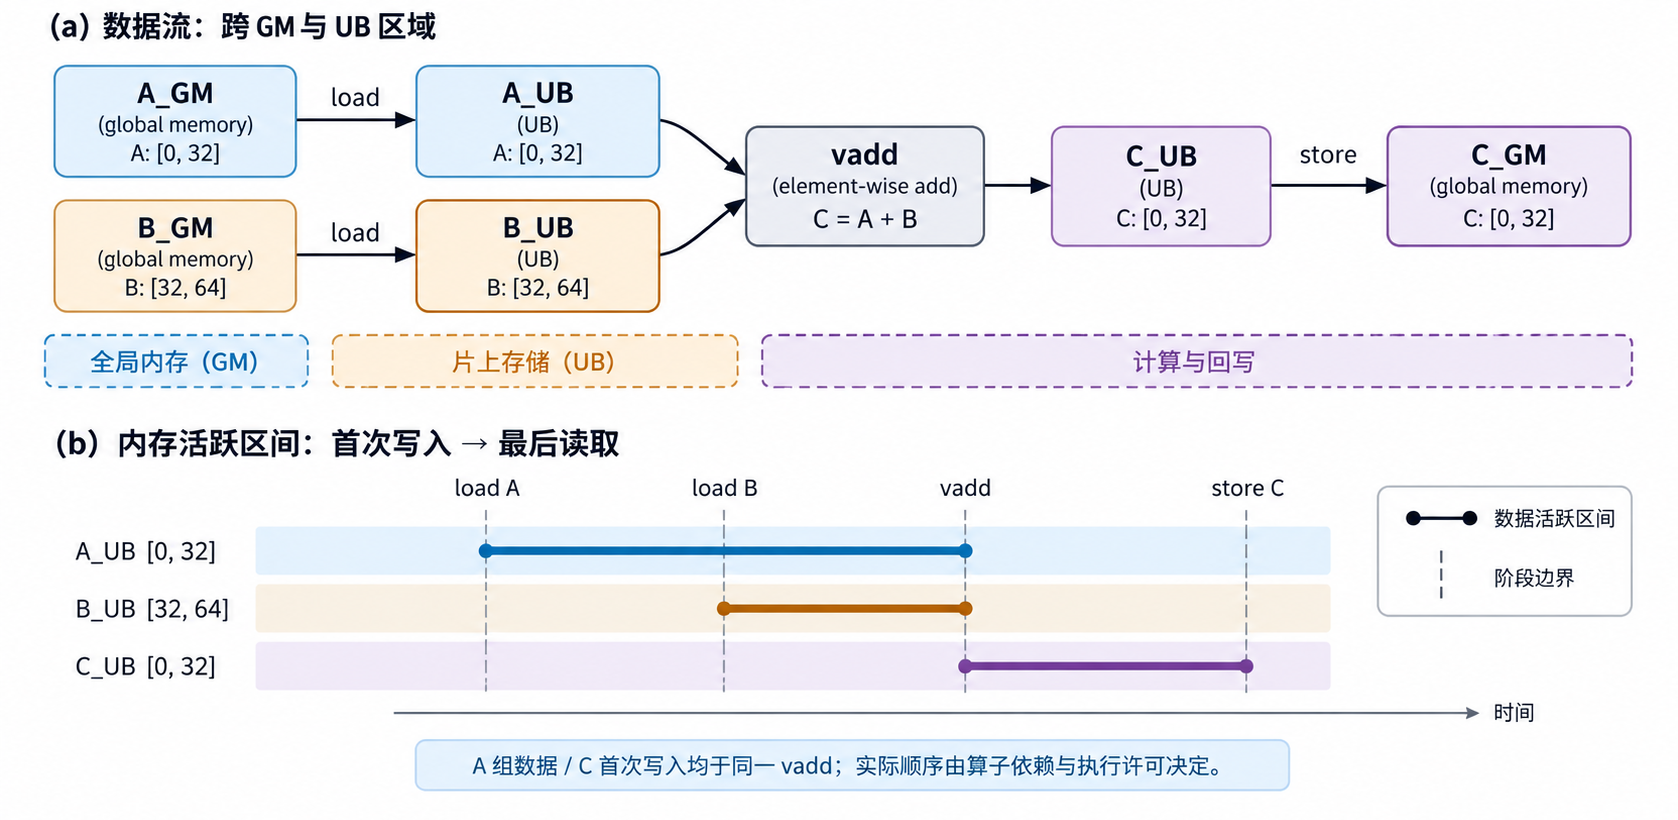
\includegraphics[width=\textwidth]{figures/fig6.png}
\caption{VecAdd 数据流和缓冲内容生命周期。区间为 UB 字节范围，横轴表示操作顺序。A 与 C 使用同一区域，并在 vadd 处共同活跃。}
\label{fig:vecadd-lifetime}
\end{figure}

A\_UB 的首次写入是 load A，最后一次读取是 vadd；B\_UB 同理。C\_UB 的首次写入也在\textbf{同一条 vadd}，最后读取是 store。在操作粒度上，输入的最后读取与输出的首次写入相遇，因此 A/C 共址的安全性还依赖该算子允许输入与输出原地重叠。

\texttt{PlanMemory.cpp}\cite{ascendplan}中，\texttt{IsReuseHIVMOp} 将无内联广播/转置的 VAdd 列入 ISA 允许原地执行的操作；\texttt{GenerateInplaceList} 在\emph{同一操作}的 gen/kill 集合中配对，要求被复用缓冲容量不小于新结果；\texttt{MergeInplaceSE} 在地址分配前合并相应存储条目。源码还检查操作数的 memref \emph{布局偏移}兼容性，这不同于最终规划的 UB 起始地址。本例具有相同形状和元素类型、各 32 字节、无广播/转置，且原 A 在 vadd 后不再读取，符合该原地复用路径。

由 use-def 关系、操作顺序及算子许可可知，本例 vadd 消费 A 后，以 C 替代其内容。上述原地复用结论仅针对本例 VAdd。静态布局使用 \texttt{[0,32)}、\texttt{[32,64)} 两段区域，相对三段独立缓冲由 96 字节减少为 64 字节；64 B 为静态 UB 布局结果，不代表设备运行时峰值或性能。偏移 0 以 UB 地址空间为基准。

\subsection{跨流水同步：从源文件顺序到 happens-before}
\label{subsec:cross-pipeline-sync}
本例 load 的 GM 至 UB 搬运属于 MTE2，vadd 属于 V，store 的 UB 至 GM 搬运属于 MTE3。它们是不同硬件流水线；IR 中 load 位于 vadd 之前，仍需同步操作保证向量流水在搬运完成后才消费数据。同步插入后的 IR 增加两对事件和末尾屏障，图\ref{fig:vecadd-pipeline}展示其依赖关系。

\begin{figure}[H]
\centering
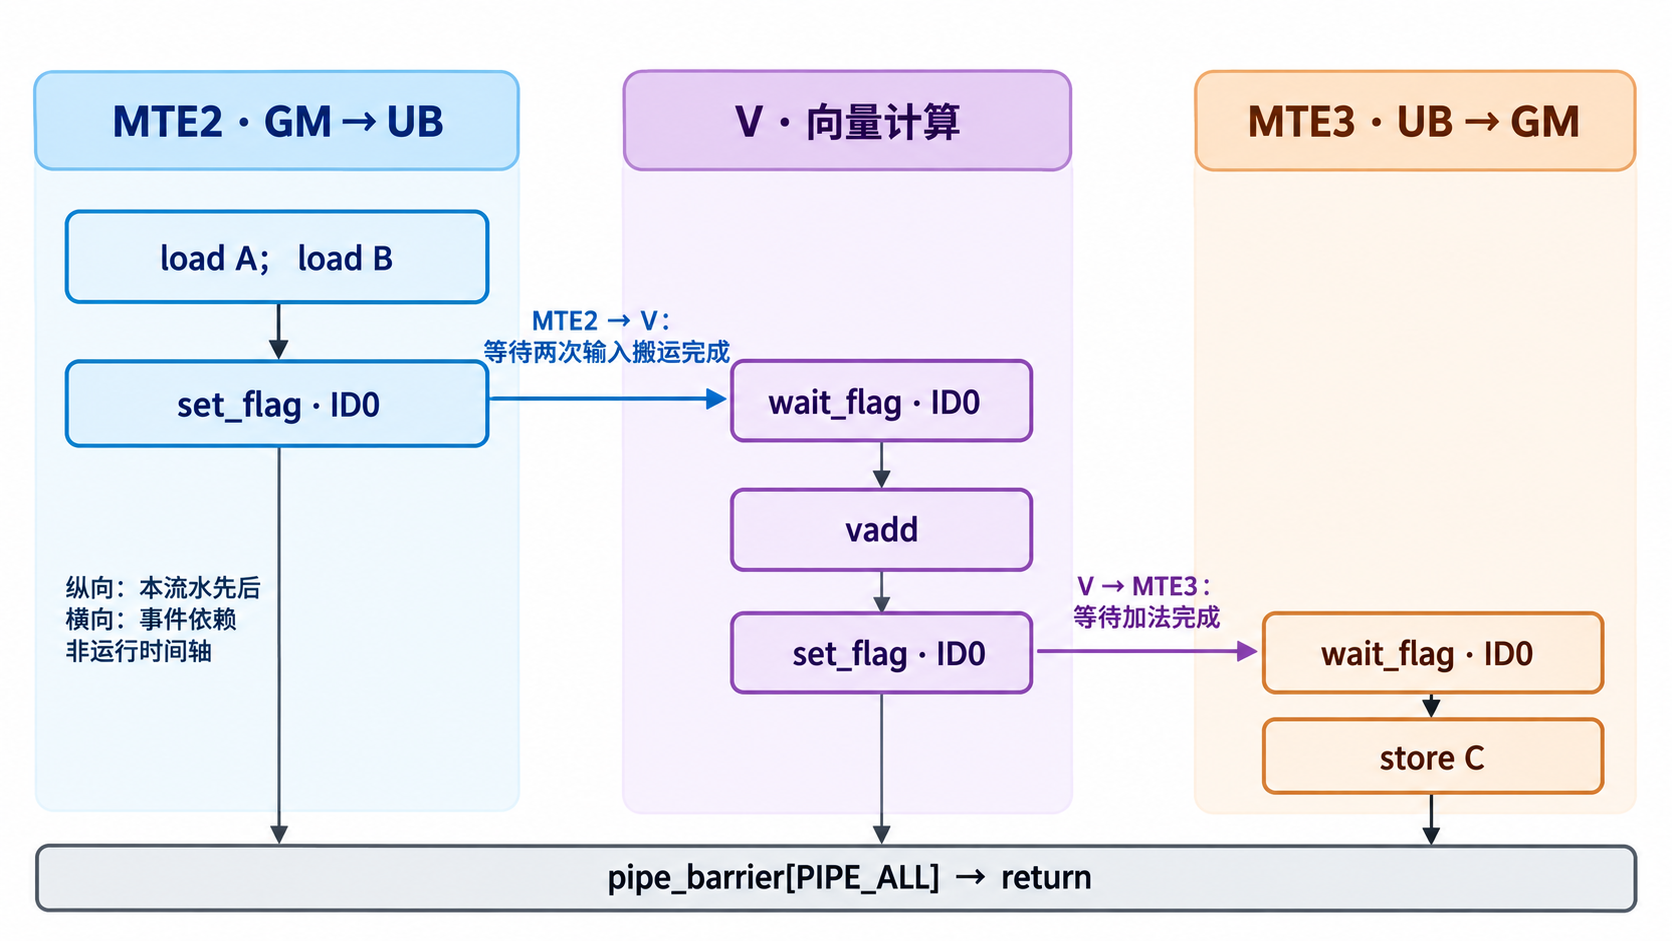
\includegraphics[width=\textwidth]{figures/fig7.png}
\caption{set/wait 配对形成的 happens-before。箭头表示流水线操作必须满足的先后关系。}
\label{fig:vecadd-pipeline}
\end{figure}

官方同步语义\cite{ascendsync}规定，\texttt{set\_flag} 等源流水前序指令完成后触发事件，\texttt{wait\_flag} 在目标流水阻塞后续指令直至事件触发。因此第一对建立“两次 load 完成 $\rightarrow$ vadd 可执行”，第二对建立“vadd 完成 $\rightarrow$ store 可执行”。两对均为 EVENT\_ID0，事件身份还包含源/目标流水：第一对为 MTE2$\rightarrow$V，第二对为 V$\rightarrow$MTE3。末尾 \texttt{pipe\_barrier[PIPE\_ALL]} 对核内所有流水施加前序完成约束，在返回处收束未完成工作；该屏障同步核内流水线，不承担多核全局同步。

\clearpage
\subsection{实际 pass 次序及其机制依赖}
\label{subsec:pass-order}
完整驱动的 \texttt{--mlir-print-ir-after-all} 输出显示以下关键顺序：核推导 $\rightarrow$ 全局 workspace 规划 $\rightarrow$ 局部 UB 规划 $\rightarrow$ \texttt{graph-sync-solver} $\rightarrow$ HIVM 模板转换；这里省略了中间其他 pass。两次 \texttt{plan-memory} 的职责不同，后一次在本例中将三个 alloc 变为 UB 偏移 0、32、0。\texttt{HIVMPipelines.cpp}\cite{ascendpipeline}中的全局规划模式、局部规划、随后同步调用及末尾模板转换与该顺序一致。

这一顺序体现了分析间的信息依赖：核推导根据设备操作约束明确 AIV，供后续设备变换使用；内存规划把逻辑缓冲落实为物理区域，使原地别名关系显式化；同步分析随后约束这些存储访问在各流水间的顺序；最后模板转换将搬运和向量操作的高层接口降为模板调用。核类型信息为设备变换提供约束，确定后的布局为同步处理提供存储访问关系。

逐步处理使用 \texttt{hivm-inject-sync}，完整驱动使用 \texttt{hivm-graph-sync-solver}；源码按选项分支选择二者。本例两条路径均产生上述关键依赖。五个逐步处理命令（含解析）与独立完整中端命令共完成六次处理，IR 重解析与关键结构一致性等 18 项检查均通过。

\subsection{模板 lowering 与后端边界}
\label{subsec:template-backend}
模板转换将两个 load、一个 vadd、一个 store 降为三类模板的四次调用：\path{load_gm_to_ubuf_1d_int16_t}、\path{vadd_1d_int16_t}、\path{store_ubuf_to_gm_1d_int16_t}。类型、实参与模板选择承接原计算；动态形状/步长的 \texttt{memref.cast} 调整调用接口。额外的第四个 \texttt{pointer\_cast} 是 vadd 的零长度临时缓冲参数，并非另一段有效数据存储。结果仍含 \texttt{func/arith/memref} 和 HIVM 同步、地址空间，\textbf{不是纯 LLVM IR}。

独立完整中端输出与驱动最终打印的模块一致。完整设备编译在外部 \texttt{hivmc} 处报告 \texttt{Cannot find hivmc under \$PATH}，\textbf{返回码为 0，且未产生 kernel.o}。驱动源码在外部后端失败后仍返回模块\cite{ascenddriver}，因此返回码 0 只反映驱动结束状态，设备编译结果还取决于诊断和目标文件。官方 host 示例仅打印 success，未逐元素校验输出。由于本地缺少 CANN/hivmc 与昇腾设备\cite{ascendfaq}，本实验完成了设备中端变换，设备 kernel 尚未生成，设备端数值正确性与性能尚未验证。


\clearpage
\section{结论}
\label{sec:conclusion}

本实验以 GCC/Clang 编译工具链、LLVM IR、RISC-V 汇编及 AscendNPU IR 为研究对象，通过编译产物分析、程序运行验证和中间表示对照，研究了源程序到目标程序的转换过程及不同抽象层次下的程序语义表示。

在完整编译流程的研究中，通过对预处理文件、LLVM IR、汇编程序和 ELF 目标文件的分析，明确了预处理、编译、汇编与链接各阶段的功能及其相互关系。不同优化配置下的实验进一步表明，编译优化不仅改变指令数量，也会重构程序的控制流和数据流。Clang 在 O2 配置下将原有循环识别为整数归约，并进行向量化、循环展开和标量尾部处理；GCC 与 Clang 在相同优化级别下则表现出不同的代码生成结果。受控对照进一步发现，向量化与展开的结构影响不能简单相加；GCC 在本例中显式启用向量化或使用 O3 仍未生成向量循环，而 Clang 的 noinline 变体因循环内保留的辅助调用未能向量化。这说明编译结果受到优化策略、编译器实现及目标架构约束的共同影响，不能仅依据优化级别或代码大小评价编译效果。

在 SysY 等价实现实验中，针对两个覆盖整数、浮点、控制流、函数和数组等语言特性的示例程序，分别构建了源语言、LLVM IR 和 RISC-V 汇编三种实现。三种实现通过相同输入及独立预期进行验证，共完成 480 次运行测试，结果全部符合预期。结合控制流图、SSA 结构和 RISC-V 调用约定的分析可以发现，源语言的语义一致性不仅依赖算术结果相同，还依赖控制流分支、短路求值的副作用、变量状态合并、数据布局和函数调用约定的正确实现。针对短路求值、有符号余数和浮点转换构造的错误变体均被测试检出，进一步验证了测试方法对这些特定语义错误的辨识能力。

在进阶实验中，通过对 AscendNPU IR VecAdd 示例的逐层 lowering 分析，观察了多级中间表示如何在保持向量加法计算语义的基础上，逐步引入设备执行所需的约束。核类型推导确定了 AIV 执行目标，内存规划将逻辑缓冲映射至 UB 地址空间，并通过满足原地执行条件的存储复用减少静态缓冲占用；跨流水同步和模板转换则进一步明确了数据搬运、向量计算及设备操作之间的依赖关系。这表明，多级中间表示不仅用于表达计算本身，也能够为面向特定硬件的存储管理和执行调度提供逐步细化的表示基础。

本实验的结论仍受到工具版本、测试输入和执行环境的限制。SysY 等价性验证覆盖的是指定有效输入域内的有限样本，不能替代完整的形式化等价证明；QEMU 执行结果不代表真实 RISC-V 硬件性能；AscendNPU IR 实验完成了主机侧中端变换，但尚未生成可执行的设备目标文件，因此不能据此判断设备端数值正确性或性能。总体而言，本实验建立了从源程序、LLVM IR、目标汇编到设备相关中间表示的分析联系，并通过可追溯的编译产物和运行结果，对不同编译阶段的功能、语义保持机制及中端 lowering 过程进行了验证。

\begingroup
\small
\begin{thebibliography}{99}
\phantomsection
\addcontentsline{toc}{section}{参考文献}
\bibitem{course} 编译原理课程．预备工作：了解你的编译器 \& LLVM IR 编程 \& 汇编编程．课程实验要求．
\bibitem{overall} 编译原理课程．上机大作业：SysY——简化 C 编译器实现总体要求．课程说明．
\bibitem{gcc} GNU Project. GCC 11.4: Overall Options. \url{https://gcc.gnu.org/onlinedocs/gcc-11.4.0/gcc/Overall-Options.html}. 访问日期：2026-10-03．
\bibitem{gccopt11} GNU Project. GCC 11.4: Options That Control Optimization. \url{https://gcc.gnu.org/onlinedocs/gcc-11.4.0/gcc/Optimize-Options.html}. 访问日期：2026-10-04．
\bibitem{llvm} LLVM Project. LLVM 14 Language Reference Manual. \url{https://releases.llvm.org/14.0.0/docs/LangRef.html}. 访问日期：2026-10-03．
\bibitem{llvmvector14} LLVM Project. Auto-Vectorization in LLVM 14. \url{https://releases.llvm.org/14.0.0/docs/Vectorizers.html}. 访问日期：2026-10-04．
\bibitem{clangremarks14} LLVM Project. Clang 14 User's Manual: optimization reports. \url{https://releases.llvm.org/14.0.0/tools/clang/docs/UsersManual.html}. 访问日期：2026-10-04．
\bibitem{riscvabi} RISC-V International. RISC-V ABIs Specification. \url{https://riscv-non-isa.github.io/riscv-elf-psabi-doc/}. 访问日期：2026-10-03．
\bibitem{riscv-isa} RISC-V International. The RISC-V Instruction Set Manual, Volume I, v20260120: \href{https://docs.riscv.org/reference/isa/v20260120/unpriv/rv64.html}{RV64I 2.1}；\href{https://docs.riscv.org/reference/isa/v20260120/unpriv/m-st-ext.html}{M 2.0}．访问日期：2026-10-04．
\bibitem{qemu} QEMU Project. User space emulator. \url{https://www.qemu.org/docs/master/user/main.html}. 访问日期：2026-10-03．
\bibitem{runtime} yuhuifishash. SysY: public compiler project, commit \path{d3639373ddc894dd0d20b307d0bf1fe92b6f685b}. \href{https://github.com/yuhuifishash/SysY/tree/d3639373ddc894dd0d20b307d0bf1fe92b6f685b}{SysY 运行库源码}．访问日期：2026-10-03．
\bibitem{sysyspec} 全国大学生计算机系统能力大赛编译系统设计赛．SysY2022 语言定义 V1；SysY2022 运行时库 V1．\href{https://github.com/william-dan/SysY2022-ARMv7-Compiler/tree/7e7778d1546b850dd720ef30fff528c18737d183}{语言与运行库定义镜像}．访问日期：2026-10-03．
\bibitem{ascendquick} Ascend. AscendNPU IR 官方快速入门．\url{https://ascendnpu-ir.gitcode.com/zh_cn/sources/introduction/quick_start/examples_zh.html}. 访问日期：2026-10-03．
\bibitem{bisheng} 华为．CANN 毕昇编译器．\url{https://www.hiascend.com/cann/bisheng}. 访问日期：2026-10-03．
\bibitem{vecadd} Ascend. AscendNPU-IR: VecAdd integration example. \href{https://github.com/Ascend/AscendNPU-IR/tree/37c6ebc33d1789500014e6a7b2b62164b3cb566b/bishengir/test/Integration/HIVM/VecAdd}{官方 VecAdd 示例}．访问日期：2026-10-03．
\bibitem{ascendfaq} Ascend. AscendNPU IR FAQ. \url{https://ascendnpu-ir.gitcode.com/en/faq/faq.html}. 访问日期：2026-10-03．
\bibitem{ascendwheel} Ascend. ascendnpu-ir 1.1.0 distribution. \url{https://pypi.org/project/ascendnpu-ir/1.1.0/}. 基于 LLVM 19.1.7，commit \texttt{428ab8fdab46}．访问日期：2026-10-03．
\bibitem{ascenddriver} Ascend. \path{BiShengIRCompileMain.cpp}, commit \path{428ab8fdab46a879c7349caba4cde705bc8c9bb6}. \href{https://github.com/Ascend/AscendNPU-IR/blob/428ab8fdab46a879c7349caba4cde705bc8c9bb6/bishengir/lib/Tools/bishengir-compile/BiShengIRCompileMain.cpp}{驱动源码（工具对应提交）}．访问日期：2026-10-03．
\bibitem{ascendplan} Ascend. \href{https://github.com/Ascend/AscendNPU-IR/blob/428ab8fdab46a879c7349caba4cde705bc8c9bb6/bishengir/lib/Dialect/HIVM/Transforms/PlanMemory.cpp}{PlanMemory.cpp}: IsReuseHIVMOp, GenerateInplaceList and MergeInplaceSE. 工具匹配提交 \texttt{428ab8fdab46}，访问日期：2026-10-04．
\bibitem{ascendsync} Ascend. \href{https://github.com/Ascend/AscendNPU-IR/blob/428ab8fdab46a879c7349caba4cde705bc8c9bb6/docs/source/zh_cn/developer_guide/features/AutoSync/AutoSync.md}{Auto-Sync: HIVM 同步操作}．同一工具匹配提交，访问日期：2026-10-04．
\bibitem{ascendpipeline} Ascend. \href{https://github.com/Ascend/AscendNPU-IR/blob/428ab8fdab46a879c7349caba4cde705bc8c9bb6/bishengir/lib/Dialect/HIVM/Pipelines/HIVMPipelines.cpp}{HIVMPipelines.cpp}．同一工具匹配提交，访问日期：2026-10-04．
\end{thebibliography}
\endgroup

\clearpage
\begingroup
\section*{附录A：实验环境与复现配置}
\phantomsection
\addcontentsline{toc}{section}{附录A：实验环境与复现配置}
\titleformat{\subsection}{\zihao{4}\bfseries}{\thesubsection}{0.75em}{}
\renewcommand{\thesubsection}{A.\arabic{subsection}}
\renewcommand{\theHsubsection}{appendix.\arabic{subsection}}
\setcounter{subsection}{0}

\subsection{实验环境与工具版本}
\label{app:environment}
表\ref{tab:environment}记录本实验实际使用的主机、交叉编译与报告工具版本；AscendNPU 专用工具的探测信息保存在 \path{artifacts/mlir/}。
\begin{table}[H]
\centering\small
\caption{实验工具与运行环境}
\label{tab:environment}
\begin{tabularx}{\textwidth}{L{3.7cm}Y}
\toprule\rowcolor{tableHead}项目 & 实测配置 \\
\midrule
操作系统 & Windows 主机；WSL2 Ubuntu 22.04.5 LTS，x86\_64，Linux 6.6.87.2 \\
本机编译器 & GCC 11.4.0；Clang / LLVM 14.0.0 \\
交叉编译器 & riscv64-linux-gnu-gcc 11.4.0；GNU Binutils 2.38 \\
汇编实验目标 & RV64GC，LP64D，Linux ELF64 RISC-V \\
运行方式 & qemu-riscv64 6.2.0 用户态模拟 \\
辅助中间表示工具 & MLIR 14.0.0；Ascend 专用工具版本另见进阶章节及环境记录 \\
报告工具 & XeTeX / TeX Live 2025；latexmk 4.87 \\
依赖来源 & Ubuntu 22.04 官方软件仓库；SysY 运行库和 AscendNPU IR 发行包 \\
\bottomrule
\end{tabularx}
\end{table}
版本记录和已安装软件包清单见 \path{artifacts/environment/versions.txt}。表中版本来自该环境记录及原报告，不代表其他机器上的安装状态。

\subsection{目标架构与实验复现}
\label{app:riscv-environment}
实验目标为 RV64GC、LP64D 与 Linux ELF64 RISC-V。SysY 的 \texttt{int} 为 32 位，指针为 64 位，浮点参数按 LP64D 硬浮点调用约定传递\cite{riscvabi}。SysY 源程序由 Clang 14 交叉编译，手写 LLVM IR 统一使用 \texttt{llvm-as-14}、\texttt{opt-14} 和 \texttt{llc-14} 验证并生成目标文件，以保持 typed-pointer IR 与 LLVM 14 工具版本兼容；手写汇编由 \texttt{riscv64-linux-gnu-gcc} 汇编，三种实现均链接相同运行库。

生成的静态 RISC-V ELF 程序由 \texttt{qemu-riscv64} 用户态模拟器执行，用于核验指令、Linux ABI 及输入输出行为，不据此推断真实硬件性能\cite{qemu}。具体依赖、构建和测试命令见仓库 README。

\paragraph{实验源码与复现资料}
实验源码与可公开的复现资料保存在公开 GitHub 仓库：\url{https://github.com/Andy3325/compiler-principles-prelab-2026}。
固定实验快照的 Commit SHA 为
\href{https://github.com/Andy3325/compiler-principles-prelab-2026/tree/39c3bca7e140bba3b800ed7d31ddb0739b5adfb1}{\nolinkurl{39c3bca7e140bba3b800ed7d31ddb0739b5adfb1}}。
仓库包含 GCC/Clang 工具链实验、两个 SysY 示例及其手写 LLVM IR 和 RISC-V 汇编、AscendNPU IR 主机侧 lowering 实验、测试与构建脚本、报告 LaTeX 源码，以及精选结果和分析记录；README 提供目录索引、环境依赖和复现步骤。第三方源码保留原许可与来源，课程原件、校徽、二进制和重复日志不随仓库分发，完整生成产物可按 README 重建。

\Needspace{18\baselineskip}
\subsection{课程要求与实验成果对应关系}
\label{app:course-results}
表\ref{tab:results-summary}给出课程要求、实验成果及正文分析位置的对应关系。
\begin{table}[H]
\centering\small
\caption{课程要求、完成结果与对应分析}
\label{tab:results-summary}
\begin{tabularx}{\textwidth}{L{3.2cm}L{2.7cm}L{2.2cm}Y}
\toprule\rowcolor{tableHead}课程要求 & 完成情况 & 对应章节 & 实验结果与证据 \\
\midrule
基本要求一：完整编译过程 & 完成 & 第\ref{sec:toolchain}节 & 预处理、汇编文本、目标文件和链接结果；六种构建，60/60 次测试通过 \\
基本要求二：三种等价实现 & 完成 & 第\ref{sec:sysy}节 & 两个 SysY 示例，静态链接运行库；480/480 次 QEMU 执行通过 \\
进阶要求：中端 lowering & 完成主机侧中端分析 & 第\ref{sec:advanced}节 & 六次处理完成，18/18 项解析与结构检查通过 \\
进阶要求：设备端执行 & 未完成 & 第\ref{sec:advanced}节\ref{subsec:template-backend} & 缺少 hivmc/CANN 与昇腾设备，未生成设备目标文件 \\
\bottomrule
\end{tabularx}
\end{table}
\endgroup

\end{document}
